\documentclass[sigconf]{acmart}
\pagestyle{plain} % removes running headers
%%
%% \BibTeX command to typeset BibTeX logo in the docs
\AtBeginDocument{%
  \providecommand\BibTeX{{%
    \normalfont B\kern-0.5em{\scshape i\kern-0.25em b}\kern-0.8em\TeX}}}

%% Rights management information.  This information is sent to you
%% when you complete the rights form.  These commands have SAMPLE
%% values in them; it is your responsibility as an author to replace
%% the commands and values with those provided to you when you
%% complete the rights form.


\copyrightyear{2021}
\acmYear{2021}
\setcopyright{acmcopyright}\acmConference[PODS '21]{Proceedings of the 40th ACM SIGMOD-SIGACT-SIGAI Symposium on Principles of Database Systems}{June 20--25, 2021}{Virtual Event, China}
\acmBooktitle{Proceedings of the 40th ACM SIGMOD-SIGACT-SIGAI Symposium on Principles of Database Systems (PODS '21), June 20--25, 2021, Virtual Event, China}
\acmPrice{15.00}
\acmDOI{10.1145/3452021.3458314}
\acmISBN{978-1-4503-8381-3/21/06}

\settopmatter{printacmref=true}%

% \copyrightyear{2021}
% \acmYear{2021}
% \setcopyright{acmcopyright}
% \acmConference[PODS '21] {Proceedings of the 40th ACM SIGMOD-SIGACT-SIGAI Symposium on Principles of Database Systems}{June 20--25, 2021}{Virtual Event, China}
% \acmBooktitle{Proceedings of the 40th ACM SIGMOD-SIGACT-SIGAI Symposium on Principles of Database Systems (PODS '21), June 20--25, 2021, Virtual Event, China}
% \acmPrice{15.00}
% \acmISBN{978-1-4503-8381-3/21/06}
% \acmDOI{10.1145/XXXXXX.XXXXXX}

\usepackage{enumitem}
\usepackage{balance}
\usepackage{xspace}

% \newcommand{\paths}{\text{PATHS}}
% % Pseudocode packages
% \usepackage{algorithm}
% \usepackage[noend]{algpseudocode}
%
% Tikz
\usepackage{tikz}
\usepackage{pgfplots}

\pgfplotsset{compat=1.12}
\usetikzlibrary{arrows,decorations.pathmorphing,backgrounds,positioning,fit,calc,automata,matrix}
\usetikzlibrary{trees}
\usetikzlibrary{shapes}
\usetikzlibrary{chains}
\usetikzlibrary{patterns}
\usetikzlibrary{tikzmark}


\usepackage{xspace}
%% commands
\newcommand{\NN}{\mathbb{N}}
\newcommand{\ZZ}{\mathbb{Z}}
\newcommand{\MM}{\mathbb{M}}
\newcommand{\SE}{\mathbb{S}}
\newcommand{\BB}{\mathbb{B}}
\newcommand{\RR}{\mathbb{R}}
\newcommand{\cF}{\mathcal{F}}
\newcommand{\cI}{\mathcal{I}}
\newcommand{\cM}{\mathcal{M}}
\newcommand{\cS}{\mathcal{S}}
\newcommand{\cX}{\mathcal{X}}
\newcommand{\cV}{\mathcal{V}}
\newcommand{\ssum}{\Sigma}
\newcommand{\sprod}{\Pi}
\newcommand{\sem}[2]{\llbracket #1 \rrbracket(#2)}
\newcommand{\Mnam}{\mathcal{M}}
\newcommand{\Mvar}{\mathcal{V}}
\newcommand{\Fun}{\mathcal{F}}
\newcommand{\Mlang}{\text{MATLANG}}
\newcommand{\llet}{\texttt{let } V = e_1 \texttt{ in } e_2}
\newcommand{\ones}{\mathbf{1}}
\newcommand{\diag}{\texttt{diag}}
\newcommand{\apply}[1]{\texttt{apply}[#1]}
\newcommand{\I}{\mathcal{I}}
\newcommand{\Voc}{\mathcal{S}}
\newcommand{\Sch}{\mathcal{S}}
\newcommand{\mtr}[1]{\textsf{Mat}[#1]}
\newcommand{\dom}{\mathcal{D}}
\newcommand{\conc}{\texttt{mat}}
\newcommand{\DD}{\texttt{Symb}}
\newcommand{\size}{\texttt{size}}
\newcommand{\ddim}{\texttt{dim}}
\newcommand{\ttype}{\texttt{type}_{\Sch}}
\newcommand{\ttypeo}{\texttt{type}_{\Sch_1}}
\newcommand{\type}{\texttt{type}}
\newcommand{\rak}{\texttt{RA}$_K^+$\xspace}
\newcommand{\lara}{\texttt{LARA}\xspace}
\newcommand{\lang}{\texttt{MATLANG}\xspace}
\newcommand{\langf}[1]{\texttt{MATLANG}[#1]}
\newcommand{\langfor}{\texttt{for}\text{-}\texttt{MATLANG}\xspace}
\newcommand{\langforf}[1]{\texttt{for}\text{-}\texttt{MATLANG}[#1]\xspace}
\newcommand{\langsum}{\texttt{sum}-\texttt{MATLANG}\xspace}
\newcommand{\langprod}{\texttt{sp}-\texttt{MATLANG}\xspace}
\newcommand{\langmprod}{\texttt{prod}-\texttt{MATLANG}\xspace}
\newcommand{\ffor}[3]{\texttt{for}\, #1,#2 \texttt{.}\, #3}
\newcommand{\initf}[4]{\texttt{for}\, #2,#3\!=\! #1 \texttt{.}\, #4}
\newcommand{\lleq}[2]{\texttt{leq}(#1,#2)}
\newcommand{\mmin}[1]{\texttt{min}(#1)}
\newcommand{\ccol}[2]{\texttt{col(}#1,#2\texttt{)}}
\newcommand{\red}[2]{\texttt{reduce(}#1,#2\texttt{)}}
\newcommand{\nneq}[2]{\texttt{neq(}#1,#2\texttt{)}}
\newcommand{\ccoleq}[2]{\texttt{col}_{\texttt{eq}}\texttt{(}#1,#2\texttt{)}}
\newcommand{\getdiag}[1]{\texttt{get{\_}diag}(#1)}
\newcommand{\diaginverse}[1]{\texttt{diag{\_}inverse}(#1)}
\newcommand{\Dist}{\texttt{Dist}}
\newcommand{\push}[2]{#1\texttt{.push}(#2)}
\newcommand{\pop}[1]{#1\texttt{.pop}}
\newcommand{\getsize}[1]{#1\texttt{.size}}
\newcommand{\gettop}[1]{#1\texttt{.top}}
\newcommand{\isplus}[1]{\texttt{isplus}\left( #1 \right)}
\newcommand{\isprod}[1]{\texttt{isprod}\left(#1 \right)}
\newcommand{\isone}[1]{\texttt{isone}\left(#1 \right)}
\newcommand{\isinput}[1]{\texttt{isinput}\left(#1 \right)}
\newcommand{\getfirst}[1]{\texttt{getfirst}\left(#1 \right)}
\newcommand{\getinput}[1]{\texttt{getinput}\left(#1 \right)}
\newcommand{\getroot}{\texttt{getroot}()}
\newcommand{\isnotlast}[2]{\texttt{not{\_}last}\left(#1,#2 \right)}
\newcommand{\nextgate}[2]{\texttt{next{\_}gate}\left(#1, #2 \right)}
\newcommand{\Iden}[1]{\texttt{Iden}(#1)}
\newcommand{\pondIden}[2]{\texttt{E}\left[ #1, #2 \right]}
\newcommand{\np}{{\sc NP}}
\newcommand{\nl}{{\sc NLOGSPACE}}
\newcommand{\logspace}{{\sc LOGSPACE}}
\newcommand{\ddom}{\mathbb{D}}
\newcommand{\fdom}{\operatorname{dom}}
\newcommand{\att}{\mathbb{A}}
\newcommand{\tuples}{\mathbf{tuples}}
\newcommand{\supp}{\operatorname{supp}}
\newcommand{\cJ}{\mathcal{J}}
\newcommand{\cR}{\mathcal{R}}
\newcommand{\adom}{\mathbf{adom}}
\newcommand{\ksum}{\oplus}
\newcommand{\kprod}{\odot}
\newcommand{\bigksum}{\bigoplus}
\newcommand{\bigkprod}{\bigodot}
\newcommand{\kzero}{\mymathbb{0}}
\newcommand{\kone}{\mymathbb{1}}
\newcommand{\row}{\mathsf{row}}
\newcommand{\rows}{\mathsf{rows}}
\newcommand{\col}{\mathsf{col}}
\newcommand{\cols}{\mathsf{cols}}
\newcommand{\arae}{Q}
\newcommand{\ssem}[2]{\llbracket #1 \rrbracket_{#2}}
\newcommand{\hadprod}{\circ} 
\newcommand{\qhadprod}{\Pi^{\hadprod}} 
\newcommand{\cA}{\mathcal{A}}
\newcommand{\arity}{\operatorname{arity}}
\newcommand{\hprod}{\circ}
\DeclareMathAlphabet{\mymathbb}{U}{BOONDOX-ds}{m}{n}
%% end macros


\begin{document}
\title{Expressive power of linear algebra query languages}
\author{Floris Geerts}
\affiliation{%
  \institution{University of Antwerp}
%  \streetaddress{P.O. Box 1212}
%  \city{Dublin}
%  \state{Ohio}
%  \postcode{43017-6221}
}
\email{floris.geerts@uantwerp.be}


\author{Thomas Mu{\~{n}}oz}
\affiliation{%
  \institution{PUC Chile and IMFD Chile}
%  \streetaddress{1 Th{\o}rv{\"a}ld Circle}
%  \city{Hekla}
%  \country{Iceland}
}
\email{tfmunoz@uc.cl}

\author{Cristian Riveros}
\affiliation{%
  \institution{PUC Chile and IMFD Chile}
%  \streetaddress{1 Th{\o}rv{\"a}ld Circle}
%  \city{Hekla}
%  \country{Iceland}
}
\email{cristian.riveros@uc.cl}

\author{Domagoj Vrgo\v{c}}
\affiliation{%
  \institution{PUC Chile and IMFD Chile}
%  \streetaddress{1 Th{\o}rv{\"a}ld Circle}
%  \city{Hekla}
%  \country{Iceland}
}
\email{dvrgoc@ing.puc.cl}

%%
%% By default, the full list of authors will be used in the page
%% headers. Often, this list is too long, and will overlap
%% other information printed in the page headers. This command allows
%% the author to define a more concise list
%% of authors' names for this purpose.
%\renewcommand{\shortauthors}{Trovato and Tobin, et al.}

%%
%% The abstract is a short summary of the work to be presented in the
%% article.
\begin{abstract}
Linear algebra algorithms often require some sort of iteration or recursion as is illustrated by standard algorithms for Gaussian elimination, matrix inversion, and transitive closure. A key characteristic shared by these 
algorithms is that they allow looping for a number of steps that is bounded by the matrix dimension. 
In this paper we extend the matrix query language \lang with this type of recursion, and show that this suffices to express  classical linear algebra algorithms. We study the expressive power of this language and show that it naturally corresponds to arithmetic circuit families, which are often said to capture linear algebra. Furthermore, we analyze several sub-fragments of our language, and show that their expressive power is closely tied to logical formalisms on semiring-annotated relations.
\end{abstract}

%%
%% Code generated by the tool at http://dl.acm.org/ccs.cfm.
%%%
\begin{CCSXML}
<ccs2012>
<concept>
<concept_id>10003752.10010070.10010111.10010113</concept_id>
<concept_desc>Theory of computation~Database query languages (principles)</concept_desc>
<concept_significance>500</concept_significance>
</concept>
<concept>
<concept_id>10003752.10003777.10003781</concept_id>
<concept_desc>Theory of computation~Circuit complexity</concept_desc>
<concept_significance>500</concept_significance>
</concept>
</ccs2012>
\end{CCSXML}

\ccsdesc[500]{Theory of computation~Database query languages (principles)}
\ccsdesc[500]{Theory of computation~Circuit complexity}
%%%
%%% Keywords. The author(s) should pick words that accurately describe
%%% the work being presented. Separate the keywords with commas.
\keywords{complexity; query languages; circuit complexity; linear algebra}
%%%
%% This command processes the author and affiliation and title
%% information and builds the first part of the formatted document.
\maketitle

\section{Introduction}
Linear algebra-based algorithms have become a key component in data analytic workflows. As such, there is a growing interest in the database community to integrate linear algebra functionalities into relational database management systems \cite{Jermaine/17/LAonRA,2019Boehm,LARA_Berlin_2016,JankovLYCZJG19,Khamis0NOS18}. In particular, from a query language perspective, several proposals have recently been put forward to unify relational algebra and linear algebra. Two notable examples of this are: \lara~\cite{HutchisonHS17}, a minimalistic language in which a number of atomic operations on 
associative tables are proposed, and \lang, a query language for 
matrices \cite{matlang,matlang-journal}.\looseness=-1

Both \lara and \lang have been studied by the database theory community, showing interesting connections to relational algebra and logic. For example, fragments of \lara are known to capture first-order logic with aggregation~\cite{BarceloH0S20}, and \lang has been recently shown to be equivalent to a restricted version of the (positive) relational algebra on $K$-relations, \rak~\cite{brijder2019matrices}, where $K$ denotes a semiring. On the other hand, 
some standard constructions in linear algebra 
are out of reach for these languages. For instance, it was shown that under standard complexity-theoretic assumptions, \lara can not compute the inverse of a matrix or its determinant~\cite{BarceloH0S20}, and operations such as the transitive closure of a matrix are known to be inexpressible in \lang~\cite{matlang-journal}. Given that these are fundamental constructs in linear algebra, one might wonder how to extend \lara or \lang in order to allow expressing such properties.

One approach would be to add these constructions explicitly to the language. Indeed, this was done for \lang in~\cite{matlang-journal}, and \lara in ~\cite{BarceloH0S20}. In these works, the authors have extended the core language with the trace, the inverse, the determinant, or the eigenvectors operators and study the expressive power of these extensions. However, one can argue that there is nothing special about these operators, apart from that they have been used historically in linear algebra textbooks and they extend the expressibility of the core language. The question here is whether these new operators form a sound and natural choice to extend the core language, or are they just some particular queries that we would like to support. 

In this paper we take a more principled approach by studying what are the atomic operations needed to define standard linear algebra algorithms. Inspecting any linear algebra textbook, one sees that most linear algebra procedures heavily rely on the use of for-loops in which iterations happen over the dimensions of the matrices involved. To illustrate this, let us consider the example of computing the transitive closure of a graph. This can be done using a modification of the Floyd-Warshall algorithm~\cite{cormen}, which takes as its input an $n\times n$ adjacency matrix $A$ representing our graph, and operates according to the following pseudo-code:
\begin{tabbing}
\quad\texttt{for}\=\,  $k = 1..n$ \texttt{do}\\
\> \texttt{for}\=\,  $i = 1..n$ \texttt{do}\\
\> \> \texttt{for}\=\,  $j = 1..n$ \texttt{do}\\
\> \> \> $A[i,j] := A[i,j] + A[i,k] \cdot A[k,j]$
\end{tabbing}
After executing the algorithm, all of the non zero entries signify an edge in the (irreflexive) transitive closure graph.

By examining standard linear algebra algorithms such as Gaussian elimination, $LU$-decomposition, computing the inverse of a matrix, or its determinant, we can readily see that this pattern continues. Namely, we observe that there are two main components to such algorithms: (i) the ability to iterate up to the matrix dimension; and (ii) the ability to access a particular position in our matrix. In order to allow this behavior in a query language, we propose to extend \lang with limited recursion in the form of for-loops, resulting in the language \langfor. To  simulate the two components of standard linear algebra algorithms in a natural way, we simulate a loop of the form \texttt{for}\, $i=1..n$ \texttt{do} by leveraging canonical vectors. In other words, we use the canonical vectors $b_1=(1,0,\ldots)$, $b_2=(0,1,\ldots)$, \ldots, to access specific rows and columns, and iterate over these vectors. In this way,
we obtain a language able to compute important linear algebra operators such as $LU$-decomposition, determinant, matrix inverse, among other things.

Of course, a natural question to ask now is whether this really results in a language suitable for linear algebra? We argue that the correct way to approach this question is to compare our language to arithmetic circuits, which have been shown to capture the vast majority of existing matrix algorithms, from basic ones such as computing the determinant and the inverse, to complex procedures such as discrete Fourier transformation, and Strassen's algorithm (see \cite{ShpilkaY10,allender} for an overview of the area), and can therefore be considered to effectively capture linear algebra. In the main technical result of this paper, we show that \langfor indeed computes the same class of functions over matrices as the ones computed by arithmetic circuit families of bounded degree.  As a consequence, \langfor inherits all expressiveness properties of circuits, and thus can simulate any linear algebra algorithm definable by circuits.

Having established that \langfor indeed provides a good basis for a linear algebra language, we move to a more fine-grained analysis of the expressiveness of its different fragments. For this, we aim to provide a connection with logical formalisms, similarly as was done by linking \lara and \lang to first-order logic with aggregates~\cite{BarceloH0S20,matlang-journal}. As we show, capturing different logics correspond to restricting how matrix variables are updated in each iteration of the for-loops allowed in \langfor. For instance, if we only allow to add some temporary result to a variable in each iteration (instead of rewriting it completely like in any programming language), we obtain a language, called \langsum, which is equivalent to \rak, directly extending an analogous result shown for \lang, mentioned earlier~\cite{brijder2019matrices}. We then study updating matrix variables based on another standard linear algebra operator, the Hadamard product, resulting in a fragment called \langprod, which we show to be equivalent to weighted logics~\cite{DrosteG05}. Finally, in \langmprod 
we update the variables based on the standard matrix product, and link this fragment 
to the ones discussed previously.  

\smallskip
\noindent
\textbf{Contribution and outline.} 
\begin{itemize}
	% [leftmargin=0.5cm]
	\item After we recall \lang in Section~\ref{sec:matlang}, we show in Section~\ref{sec:formatlang}
	how for-loops can be added to \lang in a natural way. We also observe that
	\langfor strictly extends \lang. In addition, we discuss some design decisions behind the definition of \langfor, noting that our use of canonical vectors results in the availability of an order relation.
	
	\item In Section~\ref{sec:queries} we show that \langfor can compute important linear algebra algorithms in a natural way. We provide expressions in \langfor for LU decomposition (used to solve linear systems of equations), the determinant and matrix inversion.
	\item More generally, in Section~\ref{sec:circuits} we report our main technical contribution.
	 We show that every uniform family of arithmetic circuits of polynomial degree correspond to a \langfor expression, and vice versa, when a \langfor expression has polynomial degree, then there is an equivalent uniform family of arithmetic circuits. As a consequence, \langfor inherits all expressiveness properties of such circuits.
	\item  Finally,  we generalize the semantics of \langfor to matrices with values in a semiring $K$  in Section~\ref{sec:restrict}, and show that two natural fragments of \langfor, \langsum, and \langprod, are equivalent to the (positive) relational algebra and weighted logics on binary $K$-relations, respectively. We also briefly comment on a minimal fragment of \langfor, based on \langmprod, that is able to compute matrix inversion.
\end{itemize}
Due to space limitations, we only include some proof sketches. We refer
to the full version~\cite{geerts2020expressive} for more details.

\smallskip
\noindent
\textbf{Related work.} 
We already mentioned \lara~\cite{HutchisonHS17} and \lang~\cite{matlang-journal}
whose expressive power was further analyzed in~\cite{BarceloH0S20,brijder2019matrices,Geerts19,Geerts20}.
Extensions of \texttt{SQL} for matrix manipulations are reported in~\cite{Jermaine/17/LAonRA}. Most relevant
is~\cite{JankovLYCZJG19} in which a recursion mechanism is added to \texttt{SQL} which resembles for-loops.
The expressive power of this extension is unknown, however. Classical logics with aggregation~\cite{Hella:2001} and fixed-point logics with counting~\cite{GroheP17} can also be used for linear algebra. For-loop extensions of  standard first-order logic are considered in~\cite{NevenOTB01} but with a different semantics as ours and in which no aggregation is supported.
More generally, for the descriptive complexity of linear algebra we refer to~\cite{dghl_rank,holm_phd}. Most of these works require to encode real numbers inside relations, whereas we treat real numbers as atomic values. We refer to relevant papers related to arithmetic circuits and logical formalisms on semiring-annotated relations in the corresponding sections later in the paper.

\section{MATLANG}\label{sec:matlang}
We start by recalling the matrix query language \lang, introduced in \cite{matlang-journal}, which serves as our starting point.

\smallskip
\noindent
\textbf{Syntax.}\,  Let $\Mvar = \{V_1, V_2, \ldots\}$ be a countably infinite set of \textit{matrix variables} and $\Fun=\bigcup_{k>1}\Fun_k$ with
$\Fun_k$ a set of \textit{functions} of the  form $f:\RR^k \to \RR$, where $\RR$ denotes the set of real numbers. The syntax of $\lang$ expressions is defined by the following grammar\footnote{The original syntax also permits the operator $\llet$, which replaces every occurrence of $V$ in $e_2$ with the value of $e_1$. Since this is just syntactic sugar, we omit this operator. We also explicitly include matrix addition and scalar multiplication, although these can be simulated by pointwise function applications. Finally, we use transposition instead of conjugate transposition since we work with matrices over $\RR$.}:


\begin{tabular}{lcll}
$e$ & $::=$ & $V\in \Mvar$ & (matrix variable)\\
 & $|$ & $e^T$ & (transpose)\\ 
 & $|$ & $\ones(e)$ & (one-vector)\\ 
 & $|$ & $\diag(e)$ & (diagonalization of a vector)\\  
 & $|$ & $e_1 \cdot e_2$ & (matrix multiplication)\\   
 & $|$ & $e_1 + e_2$ & (matrix addition)\\   
 & $|$ & $e_1\times e_2$ & (scalar multiplication)\\
 & $|$ & $f(e_1,\ldots ,e_k)$ & (pointwise application of $f\in\Fun_k$).    
\end{tabular}
\vspace{1ex}

$\lang$ is parametrized by a collection of functions $\Fun$ but in the remainder of the paper we only make this dependence explicit, and write $\langf{\Fun}$, for some set $\Fun$ of functions, when these functions are crucial for some results to hold. When we simply write \lang, we mean that any function can be used (including not using any function at all).

When working with \lang\ expressions throughout the paper, we assume the expression $e$ to be given by its parse tree. Alternatively, we can assume the expression to be fully parenthesized. This allows us to disambiguate expressions of the form $A + B\cdot C$, since the parse tree (or the parentheses) will tell us whether we are working with $(A) + (B\cdot C)$, or with $(A+B)\cdot C$. For the sake of brevity, throughout the paper we will also sometimes revert to usual operator precedence syntax, assuming matrix and scalar multiplication to have precedence over the sum (the precedence of the other operators is always unambiguous). This means that when we write $A + B\cdot C$, we are actually referring to $(A) + (B\cdot C)$.

\smallskip
\noindent
\textbf{Schemas and typing.}\,
To define the semantics of \lang\ expressions we need a notion of schema and well-typedness of expressions. A \lang\ \textit{schema} $\Sch$ is a pair $\Sch=(\Mnam,\size)$, where $\Mnam\subset \Mvar$ is a finite set of matrix variables, and $\size: \Mnam \mapsto \DD\times \DD$ is a function that maps each matrix variable in $\Mnam$ to a pair of \textit{size symbols}. The $\size$ function helps us determine whether certain matrix operations, such as matrix multiplication, can be performed for matrices adhering to a schema. 
We denote size symbols by Greek letters $\alpha,\beta,\gamma$. We also assume that $1\in \DD$. 
To help us determine whether a \lang\ expression can always be evaluated, we define the \textit{type} of an expression $e$, with respect to a schema $\Sch$, denoted by $\ttype(e)$, inductively as follows:
\begin{itemize}
\item $\ttype(V):= \size(V)$, for a matrix variable $V\in\Mnam$;
\item $\ttype(e^T):= (\beta,\alpha)$ if $\ttype(e)=(\alpha,\beta)$;
\item $\ttype(\ones(e)):= (\alpha,1)$ if $\ttype(e)=(\alpha,\beta)$;
\item $\ttype(\diag(e)):= (\alpha,\alpha)$, if $\ttype(e)=(\alpha,1)$;
\item $\ttype(e_1 \cdot e_2):= (\alpha,\gamma)$ if  $\ttype(e_1)=(\alpha,\beta)$, and $\ttype(e_2)=(\beta,\gamma)$;
\item $\ttype(e_1 + e_2):=(\alpha,\beta)$ if $\ttype(e_1)=\ttype(e_2)=(\alpha,\beta)$;
\item $\ttype(e_1\times e_2):=(\alpha,\beta)$ if $\ttype(e_1)=(1,1)$ and $\ttype(e_2)=(\alpha,\beta)$; and
\item $\ttype(f(e_1,\ldots ,e_k)):= (\alpha,\beta)$, whenever $\ttype(e_1) = \cdots = \ttype(e_k) := (\alpha,\beta)$ and $f\in\Fun_k$.
\end{itemize}
We call an expression \textit{well-typed} according to the schema $\Sch$, if it has a defined type. 
A well-typed expression can be evaluated regardless of the actual sizes of the matrices assigned to matrix variables, as we describe next.

We will usually work with matrices with different sizes (i.e., ``rectangular matrices''), but sometimes it will be helpful to restrict to ``square matrices''. For this we say that $\Sch$ is a schema over square matrices if there exists $\alpha$ such that each variable has type $(\alpha,\alpha),(\alpha,1),(1,\alpha)$, or $(1,1)$. This restriction will be useful when comparing the expressiveness of our proposal with other formalisms (e.g., see Section~\ref{sec:restrict}). 

\smallskip
\noindent
\textbf{Semantics.}\, We use $\mtr{\RR}$ to denote the set of all real matrices and for 
$A\in\mtr{\RR}$, $\dim(A)\in\NN^2$ denotes its dimensions.
A (\lang) \textit{instance} $\I$ over a schema$\Sch=(\Mnam,\size)$ is a pair $\I = (\dom,\conc)$, where $\dom : \DD \mapsto \NN$ assigns a value to each size symbol (and thus in turn  dimensions to each matrix variable), and $\conc : \Mnam \mapsto \mtr{\RR}$ assigns a concrete matrix to each matrix variable $V\in \Mnam$, such that $\dim(\conc(V)) = \dom(\alpha)\times \dom(\beta)$ if $\size(V) = (\alpha,\beta)$. That is, an instance tells us the dimensions of each matrix variable, and also the concrete matrices assigned to the variable names in $\Mnam$. Notice that having the function $\dom$ allows us to specify when two matrix variables have to be assigned matrices of the same dimension. We assume that $\dom(1) = 1$, for every instance $\I$. If $e$ is a well-typed expression according to $\Sch$, then we denote by $\sem{e}{\I}$ the matrix obtained by evaluating $e$ over $\I$, and define it as follows\footnote{We also use easily definable operations as matrix minus ($-$) and assume the existence of some constants (such as $[1]$) in $\Mnam$. Additionally, several times we omit the $\times$ operator to weigh expressions.}:
\begin{itemize}
\item $\sem{V}{\I} := \conc(V)$, for $V\in \Mnam$;
\item $\sem{e^T}{\I} := \sem{e}{\I}^T$, where $A^T$ is the transpose of matrix $A$;
\item $\sem{\ones(e)}{\I}$ is a $n\times 1$ vector with $1$ as all of its entries, where $\dim(\sem{e}{\I})=(n,m)$;
\item $\sem{\diag(e)}{\I}$ is a diagonal matrix with the vector $\sem{e}{\I}$ on its main diagonal, and zero in every other position;
\item $\sem{e_1\cdot e_2}{\I} := \sem{e_1}{\I} \cdot \sem{e_2}{\I}$;
\item $\sem{e_1+ e_2}{\I} := \sem{e_1}{\I} + \sem{e_2}{\I}$;
\item $\sem{e_1\times e_2}{\I} := a\times \sem{e_2}{\I}$ with $\sem{e_1}{\I}=[a]$; and
\item $\sem{f(e_1,\ldots ,e_k)}{\I}$ is a matrix $A$ of the same size as $\sem{e_1}{\I}$, and where $A_{ij}$ has the value $f(\sem{e_1}{\I}_{ij},\ldots ,\sem{e_k}{\I}_{ij})$.
\end{itemize}

\noindent
Although \lang\ forms a solid basis for a matrix query language, it is limited in expressive power. Indeed, \lang\ is subsumed by first order logic with aggregates that uses only three variables \cite{matlang-journal}. 
Hence, no \lang\ expression exists that can compute the transitive closure of a graph (represented by its adjacency matrix) or can compute the inverse of a matrix. Rather than extending \lang\ with specific linear algebra operators, such as matrix inversion, we  
next introduce a limited form of recursion in \lang.

\section{Extending MATLANG with for loops}\label{sec:formatlang}
To extend \lang\ with recursion, we take inspiration from classical linear algebra algorithms, such as those described in \cite{num}. Many of these algorithms are based on \textit{for-loops} in which the termination condition for each loop is determined by the matrix dimensions. We have seen how the transitive closure of a matrix can be computed using for-loops in the Introduction. Here we add this ability to \lang, and show that the resulting language, called $\langfor,$ can compute properties outside of the scope of \lang. We see more advanced examples, such as Gaussian elimination and matrix inversion, later in the paper. 

\subsection{Syntax and semantics of \langfor} The syntax of \langfor is defined just as for \lang but with an extra rule in the grammar:
\medskip

\begin{tabular}{lcll}
 $\ffor{v}{X}{e}$ & (canonical for loop, with $v, X \in \Mvar$). 
\end{tabular}

\medskip
\noindent Intuitively, $X$ is a matrix variable which is iteratively updated according to the expression $e$. We simulate iterations of the form ``\texttt{for} $i\in [1..n]$'' by letting $v$ loop over the \textit{canonical vectors} $b_1^n,\ldots,b_n^n$ of dimension $n$. Here,
$b_1^n = [1\ 0 \cdots 0]^T$, $b_2^n = [0\ 1\ 0 \cdots 0]^T$, etc. When $n$ is clear from the context we simply write $b_1,b_2,\ldots$. In addition, the expression $e$ in the rule above may depend on $v$. 

We next make the semantics precise and start by
declaring the type of loop expressions.
Given a schema $\Sch=(\Mnam,\size)$, the type of a \langfor expression $e$, denoted $\ttype(e)$, is defined inductively as in \lang but with following extra rule:
\begin{itemize}
\item $\ttype(\ffor{v}{X}{e}) := (\alpha,\beta)$, if \\
$\ttype(e)=\ttype(X) =(\alpha,\beta)$ and $\ttype(v) = (\gamma,1)$.
\end{itemize}
We note that $\Sch$ now necessarily includes $v$ and $X$ as variables and assigns size symbols to them.
We also remark that in the definition of the type of $\ffor{v}{X}{e}$, we require that $\ttype(X) = \ttype(e)$ as this expression updates the content of the variable $X$ in each iteration using the result of $e$. We further restrict the type of 
$v$ to be a vector, i.e., $\ttype(v)=(\gamma,1)$, since $v$ will be instantiated with canonical vectors.
A \langfor\ expression $e$ is well-typed over a schema $\Sch=(\Mnam,\size)$ if its type is defined. 

For well-typed expressions we next define their semantics. This is done in an inductive way, just as for \lang. To define the semantics of $\ffor{v}{X}{e}$ over an instance $\I$, we need the following notation. Let $\I$ be an instance and $V\in \Mnam$. Then $\I[V_1 := A_1, \ldots, V_l:=A_l]$ denotes an instance that coincides with $\I$, except that the value of the matrix variable $V_i$ is given by the matrix $A$, for $i\in\lbrace 1, \ldots, l\rbrace$. Assume that
$\ttype(v)= (\gamma,1)$, and $\ttype(e) = (\alpha,\beta)$ and $n := \dom(\gamma)$. Then, $\sem{\ffor{v}{X}{e}}{\I}$ is defined iteratively, as follows:
\begin{itemize}
\item Let $A_0 := \mathbf{0}$ be the zero matrix of size $\dom(\alpha)\times \dom(\beta)$.
\item For $i=1,\ldots n$, compute $A_i:= \sem{e}{\I[v := b^{n}_i, X:= A_{i-1}]}$.
\item Finally, set $\sem{\ffor{v}{X}{e}}{\I}:= A_{n}$.
\end{itemize}

For better understanding how \langfor  works, we next provide some  examples.
We start by showing that the one-vector and $\diag$ operators are redundant
in \langfor.
\begin{example}\label{ex:onevec}
We first show how the one-vector operator $\ones(e)$ can be expressed using \texttt{for} loops.
It suffices to consider the expression
$$e_{\ones}:=\ffor{v}{X}{X+v},$$
with $\ttype(v)=(\alpha,1)=\ttype(X)$ if $\ttype(e)=(\alpha,\beta)$. This expression is well-typed
and is of type $(\alpha,1)$. When evaluated over some instance $\I$ with $n=\dom(\alpha)$, $\sem{e_{\ones}}{\I}$ is defined as follows.
Initially, $A_0:=\mathbf{0}$. Then $A_i:=A_{i-1}+b_i^n$, i.e., the $i$th canonical vector is added to $A_{i-1}$.
Finally, $\sem{e_{\ones}}{\I}:=A_n$ and this now clearly coincides with $\sem{\ones(e)}{\I}$.\qed
\end{example}

\begin{example}\label{ex:diag}
We next show that the $\diag$ operator is redundant in \langfor.
Indeed, it suffices to consider the expression
$$e_{\mathsf{diag}}:=
\ffor{v}{X}{X + (v^T\cdot e) \times v\cdot v^T},$$ where $e$ is a \langfor\  expression of type $(\alpha,1)$. For this expression to be well-typed, $v$ has to be a vector variable of type $\alpha\times 1$ and $X$ a matrix variable of type $(\alpha,\alpha)$. Then, $\sem{e_{\mathsf{diag}}}{\I}$ is defined as follows.
Initially, $A_0$ is the zero matrix of dimension $n\times n$, where $n=\dom(\alpha)$. Then, in each iteration
$i\in[1..n]$, $A_{i}:=A_{i-1}+  ((b_i^n)^T\cdot\sem{e}{\I})\times (b_i^n\cdot (b_i^n)^T)$. In other words, $A_i$ is obtained by adding the matrix with value $(\sem{e}{\I})_i$ on position $(i,i)$ to $A_{i-1}$. Hence, $\sem{e_{\mathsf{diag}}}{\I}:=A_n=\sem{\diag(e)}{\I}$.\qed
 \end{example}

These examples illustrate that we can limit \langfor to consist of the following ``core'' operators: transposition, matrix multiplication and addition, scalar multiplication, pointwise function application, and for-loops. More specific, \langfor is defined by the following simplified syntax:
$$
e ::= V \ \mid \ e^T \!\ \mid \ e_1 \cdot e_2 \ \mid \ e_1 + e_2 \ \mid \ e_1\times e_2  \ \mid \  f(e_1,\ldots ,e_k) \ \mid \ \ffor{v}{X}{e}
$$
Similarly as for \lang, we write $\langforf{\Fun}$ for some set $\Fun$ of functions when these are required for the task at hand.

As a final example, we show that we can compute whether a graph contains a 4-$\textsf{clique}$ using \langfor.
\begin{example}\label{ex:fourcliques}
To test for $4$-cliques it suffices to consider the following expression with for-loops nested four times:
\begin{tabbing}
\texttt{for\,}\=$u,\,X_1.\ \ X_1 \ + $\\
\> \texttt{for\,}\=$v,\,X_2.\ \ X_2 \ +$ \\
\>\>\texttt{for\,}\=$w,\,X_3.\ \ X_3 \ +$ \\
\>\>\>\texttt{for\,}\=$x,\,X_4.\ \ X_4 \ +$ \\
\>\>\>\>$u^T\cdot V\cdot v \cdot u^T\cdot V\cdot w\cdot u^T\cdot V\cdot x \cdot $\\
\>\>\>\>$v^T\cdot V\cdot w \cdot v^T\cdot V\cdot x\cdot w^T\cdot V\cdot x \cdot g(u,v,w,x)$
\end{tabbing}
with $g(u,v,w,x)=f(u,v)\cdot f(u,w)\cdot f(u,x)\cdot f(v,w)\cdot f(v,x)\cdot f(w,x)$ and
$f(u,v)=1-u^T\cdot v$. Note that $f(b_i^n,b_j^n)=1$ if $i\neq j$ and $f(b_i^n,b_j^n)=0$ otherwise.
Hence, $g(b_i^n,b_j^n,b_k^n,b_\ell^n)=1$ if and only if all $i,j,k,l$ are pairwise different.
When evaluating the expression on an instance $\I$ such that $V$ is assigned to the adjacency 
matrix of a graph, the expression above evaluates to a non-zero value if and only if the graph
contains a four-clique.\qed
\end{example}

Given that \lang can not check for 4-cliques \cite{matlang-journal}, we easily obtain the following.

\begin{proposition}
\label{cor-ml-fml}
For any collection of functions $\Fun$, 
$\langf{\Fun}$ is properly subsumed by $\langforf{\Fun}$.
\end{proposition} 

\subsection{Design decisions behind \langfor}
\noindent\textbf{Loop Initialization.} As the reader may have observed, in the semantics of for-loops we 
always initialize $A_0$ to the zero matrix~$\mathbf{0}$ (of appropriate dimensions). It is often convenient
to start the iteration given some concrete matrix  originating from the result of evaluation a \langfor\ expression $e_0$. To make this explicit, we write $\initf{e_0}{v}{X}{e}$ and its semantics is defined as above
with the difference that $A_0:=\sem{e_0}{\I}$. We observe, however, that $\initf{e_0}{v}{X}{e}$ can already
be expressed in \langfor. In other words, we do not loose generality by assuming an initialization of $A_0$ by $\mathbf{0}$.
The key insight is that in \langfor\ we can check during evaluation whether or not
the current canonical vector $b_i^n$ is equal to $b_1^n$. This 
is due to the fact that for-loops iterate over the canonical vectors in a fixed order. We discuss this more in the next paragraph.
In particular, we can define a \langfor expression $\mmin$, which when evaluated on an instance, returns $1$ if its input vector is $b_1^n$, and returns $0$ otherwise. Given $\mmin$, consider now the
\langfor\ expression
 $$\ffor{v}{X}{\mmin{v}\cdot e(v,X/e_0) + (1-\mmin{v})\cdot e(v,X)},$$
 where we explicitly list $v$ and $X$ as matrix variables on which $e$ potentially depends on, and where
 $e(v,X/e_0)$ denotes the expression obtained by replacing every occurrence of $X$ in $e$ with $e_0$.
When evaluating this expression on an instance $\I$, $A_0$ is initial set to the zero matrix, in the first iteration (when  $v=b_1^n$ and thus $\mmin{v}=1$)
we have $A_1=\sem{e}{\I[v:=b_1^n,X:=\sem{e_0}{\I}]}$, and for consecutive iterations (when only the part related to $1-\mmin{v}$ applies) $A_i$ is updated as before. Clearly, the result of this evaluation is equal to
$\sem{\initf{e_0}{v}{X}{e}}{\I}$. 


As an illustration, we consider the Floyd-Warshall algorithm given in the Introduction. 

\begin{example}\label{ex:floyd}
Consider the following expression:
\begin{tabbing}
$e_{FW} := $ \texttt{for\,}\=$v_k,\, X_1\!=\!A.\ \ X_1 \ + $\\
\> \texttt{for\,}\=$v_i, \, X_2.\ \ X_2 \ +$ \\
\>\>\texttt{for\,}\=$v_j,\, X_3.\ \ X_3 \ +$ \\
\>\>\>$(v_i^T\cdot X_1\cdot v_k \cdot v_k^T\cdot X_1\cdot v_j)\times v_i\cdot v_j^T$
\end{tabbing}
The expression $e_{FW}$ simulates the Floyd-Warshall algorithm by updating the matrix $A$, which is stored in the variable $X_1$. The inner sub-expression here constructs an $n\times n$ matrix that contains one in the position $(i,j)$ if and only if one can reach the vertex $j$ from $i$ by going through $k$, and zero elsewhere. If an instance $\I$ assigns to $A$ the adjacency matrix of a graph, then $\sem{e_{FW}}{\I}$ will be equal to the matrix produced by the algorithm given in the Introduction.
\qed
\end{example}


\noindent\textbf{Order.} By introducing for-loops we not only extend \lang\ with bounded recursion, we also introduce order information. Indeed, the semantics of the \texttt{for} operator assumes that the canonical vectors $b_1,b_2,\ldots$
are accessed in this order. It implies, among other things, that \langfor\ expressions are not permutation-invariant.
We can, for example, return the bottom right-most entry in a matrix. Indeed, consider the expression $e_{\mathsf{max}} := \ffor{v}{X}{v}$ which, for it to be well-typed, requires both $v$ and $X$ to be of type $(\alpha,1)$. Then, $\sem{e_{\mathsf{max}}}{\I}=b_n^n$, for $n=\dom(\alpha)$, simply because initially, $X=\mathbf{0}$, but $X$ will be overwritten by $b_1^n,b_2^n,\ldots,b_n^n$, in this order. Hence, at the end of the evaluation $b_n^n$ is returned.
To extract the bottom right-most entry from a matrix, we now simply use $e_{\mathsf{max}}^T\cdot V\cdot e_{\mathsf{max}}$.

Although the order is implicit in \langfor, we can explicitly use this order in \langfor expressions. More precisely, the order on canonical vectors is made accessible by
using the matrix:
\[
S_{\leq} = \begin{bmatrix}
1 & 1 & \cdots &  1 \\
0 & 1 & \cdots & 1\\
\vdots & \vdots & \ddots & 1 \\
0 & 0 & \cdots & 1 
\end{bmatrix}.
\] 
We observe that $S_{\leq}$ has the property that $b_i^T\cdot S_{\leq} \cdot b_j=1$, for two canonical vectors $b_i$ and $b_j$ of the same dimension, if and only if $i\leq j$. Otherwise, $b_i^T\cdot S_{\leq} \cdot b_j=0$. 
Interestingly, we can build the matrix $S_{\leq}$ with the following \langfor expression:
$$
e_{\leq}=\ffor{v}{X}{X + \left((X\cdot e_{\mathsf{max}}) + v \right)\cdot v^T + v\cdot e^T_{\mathsf{max}}},
$$
where $e_{\mathsf{max}}$ is as defined above. The intuition behind this expression is that by using the last canonical vector $b_n$, as returned by $e_{\mathsf{max}}$, we have access to the last column of $X$ (via the product $X\cdot e_{\mathsf{max}}$). We use this column such that after the $i$-th iteration, this column contains the $i$-th column of $S_{\leq}$. This is done by incrementing $X$ with $v\cdot e_{\mathsf{max}}^T$.
To construct $S_{\leq}$, in the $i$-th iteration we further increment $X$ with 
(i)~the current last column in $X$ (via $X\cdot e_{\mathsf{max}}\cdot v^T$) which holds
the $(i-1)$-th column of $S_{\leq}$; and (ii)~the current canonical vector (via $v\cdot v^T$). Hence, after iteration $i$, $X$ contains the first $i$ columns of $S_{\leq}$ and holds the $i$th column of $S_{\leq}$ in its last column. It is now readily verified that $X=S_{\leq}$ after the $n$th iteration.

It should be clear that if we can compute $S_{\leq}$ using $e_{\leq}$, then we can easily define the following predicates and vectors related with the order of canonical vectors:
\begin{itemize}
	\item $\mathsf{succ}(u,v)$ such that $\mathsf{succ}(b_i^n,b_j^n)=1$ if $i\leq j$ and $0$ otherwise. Similarly, we can define
	$\mathsf{succ}^+(u,v)$ such that  $\mathsf{succ}^+(b_i^n,b_j^n)=1$ if $i < j$ and $0$ otherwise;
	\item $\mathsf{min}(u)$ such that  $\mathsf{min}(b_i^n)=1$ if $i=1$ and $\mathsf{min}(b_i^n)=0$ otherwise; 
	\item $\mathsf{max}(u)$ such that  $\mathsf{max}(b_i^n)=1$ if $i=n$ and $\mathsf{min}(b_i^n)=0$ otherwise; and
	\item $e_{\mathsf{min}}$ and $e_{\mathsf{max}}$ such that $\sem{e_{\mathsf{min}}}{\I}=b_1^n$ and 
	$\sem{e_{\mathsf{max}}}{\I}=b_n^n$, respectively.
\end{itemize}
We refer to the full version~\cite{geerts2020expressive} for details.

Having order information available results in \langfor to be quite expressive. We heavily rely on order information in the next sections to compute the inverse of matrices and more generally to simulate low complexity Turing machines and arithmetic circuits.

\section{Algorithms in Linear Algebra}\label{sec:queries}
One of our main motivations to introduce for-loops is to be able
to express classical linear algebra algorithms in a natural way. We have seen that \langfor is
quite expressive as it can check for cliques, compute the transitive closure, and can even
leverage a successor relation on canonical vectors. The big question is how expressive \langfor
actually is. We will answer this in the next section by connecting \langfor with 
arithmetic circuits of polynomial degree. Through this connection, one can move back and forth between \langfor and arithmetic circuits, and as a consequence, anything computable by such a circuit can be
computed by \langfor as well. When it comes to specific linear algebra algorithms, the detour via circuits
can often be avoided. Indeed, in this section we illustrate that \langfor is able to
compute LU decompositions of matrices. These decompositions form the basis of many other algorithms, such as solving linear systems of equations. We further show that \langfor is expressive enough to compute matrix inversion and the determinant. We recall that matrix inversion and determinant need to be explicitly added as separate operators in \lang~\cite{matlang-journal} and that the LARA language is unable to invert matrices under usual complexity-theoretic assumptions~\cite{BarceloH0S20}.

\subsection{LU decomposition}
A lower-upper (LU) decomposition factors a matrix $A$ as the product of a lower triangular matrix $L$ and upper triangular matrix $U$.  
This decomposition, and more generally LU decomposition with row pivoting (PLU),  underlies many linear algebra algorithms and 
we next show that \langfor can compute these decompositions.

\smallskip
\noindent
\textbf{LU decomposition by Gaussian elimination.} LU decomposition can be seen as a matrix form of Gaussian elimination in which the columns of $A$
are reduced, one by one, to obtain the matrix $U$. The reduction of columns of $A$ is achieved
as follows. Consider the first column $[A_{11},\ldots,A_{n1}]^T$ of $A$ and  define 
$c_1 := [0, \alpha_{21},\ldots, \alpha_{n1}]^T$ 
with $\alpha_{j1} := -\frac{A_{j1}}{A_{11}}$. Let $T_1:=I+ c_1\cdot b_1^T$ and consider
$T_1\cdot A$. That is, the $j$th row of $T_1\cdot A$ is obtained by multiplying the first row of $A$ by $\alpha_{j1}$ and adding it to the $j$th row of $A$. As a result, the first column of $T_1\cdot A$ is equal to $[A_{11},0,\ldots,0]^T$, i.e., 
all of its entries below the diagonal are zero.  One then iteratively performs a similar computation, using a matrix $T_i:=I+c_i\cdot b_i^T$, where $c_i$ now depends on the $i$th column in $T_{i-1}\cdots T_1\cdot A$. As a consequence, $T_i\cdot T_{i-1}\cdots T_1\cdot A$ is upper triangular
in its first $i$ columns. At the end of this process, $T_n\cdots T_1\cdot A=U$ where $U$ is the desired upper triangular matrix.
Furthermore, it is easily verified that each $T_i$ is invertible and by defining $L:=T_1^{-1}\cdot\cdots\cdot T_n^{-1}$ one obtains a lower triangular matrix satisfying $A=L\cdot U$. The above procedure is only successful when the denominators used in the definition of the vectors $c_i$ are non-zero. When this is the case we call a matrix $A$ \textit{LU-factorizable}. 

In case when such a denominator is zero in one of the reduction steps, one can remedy this situation by \textit{row pivoting}. That is, when the $i$th entry of the
$i$th row in $T_{i-1}\cdots T_1\cdot A$ is zero, one replaces the $i$th row by  $j$th row in this matrix, with $j>i$, provided that the $i$th entry of the $j$th row is non-zero. If no such row exists, this implies that all elements below the diagonal are zero already in column $i$ and one can proceed with the next column. One can formulate this in matrix terms by stating that there exists a permutation matrix $P$, which pivots rows, such that $P\cdot A=L\cdot U$. Any matrix $A$ is LU-factorizable \textit{with pivoting}.

\smallskip
\noindent
\textbf{Implementing LU decomposition in \langfor.} 
We first assume that the input matrices are LU-factorizable. We deal with general matrices later on.
To implement the above procedure, we need to compute the vector $c_i$ for each column $i$. We do this in two steps. First, we extract from our input matrix its $i$th column and set all its upper diagonal entries to zero
by means of 
 the 
 expression:
$$\ccol{V}{y} := \ffor{v}{X}{\mathsf{succ}^+(y,v)\cdot(v^T\cdot V \cdot y)\cdot v + X}.$$
Indeed, when $V$ is assigned to a matrix $A$ and $y$ to $b_i$, we have that $X$ will be initially assigned
$A_0=\mathbf{0}$ and in consecutive iterations,  $A_j=A_{j-1}+ b_j^T\cdot A\cdot b_i$ if $j>i$ (because $\mathsf{succ}^+(b_i,b_j)=1$ if $j>i$) and $A_j=A_{j-1}$ otherwise (because $\mathsf{succ}^+(b_i,b_j)=0$ for $j\leq i$). The result of this evaluation is the desired column vector.
Using $\ccol{V}{y}$, we can now compute $T_i$ by the following expression:
$$\red{V}{y} := e_{\mathsf{Id}}+ f_/(\ccol{V}{y},-(y^T\cdot V\cdot y)\cdot \ones(y))\cdot y^T,$$
where $f_/:\RR^2\to\RR:(x,y)\mapsto x/y$ is the division function\footnote{We set division by zero to zero.}. 
When $V$ is assigned to $A$ and $y$ to $b_i$, $f_/(\ccol{A}{b_i},-(b_i^T\cdot A\cdot b_i)\cdot \ones(b_i))$ is equal to the vector $c_i$ used in the definition of $T_i$. To perform the reduction steps for all columns, we consider
the expression:
$$
e_{U}(V) :=  \left( \initf{e_{\mathsf{Id}}}{y}{X}{\red{X\cdot V}{y}\cdot X} \right) \cdot V.
$$
That is, when $V$ is assigned $A$, $X$ will be initially $A_0=e_{\mathsf{Id}}$, and then
$A_i=\red{A_{i-1}\cdot A}{b_i}=T_i\cdot T_{i-1}\cdots T_1\cdot A$, as desired.
One can show, see~\cite{geerts2020expressive} for details, that because we can obtain the matrices $T_i$ in \langfor and that these
are easily invertible, we can also construct an expression $e_L(V)$ which evaluates to $L$ when $V$ is assigned to
$A$. We may thus conclude the following.
\begin{proposition}\label{prop:gauss}
There exists $\langforf{f_/}$ expressions $e_L(V)$ and $e_U(V)$ such that
$\sem{e_L}{\I}=L$ and $\sem{e_U}{\I}=U$ form an LU-decomposition of $A$,
where $\conc(V)=A$ and $A$ is LU-factorizable.\qed
\end{proposition}
We remark that the proposition holds when division is added as a function in $\Fun$
in \langfor. When row pivoting is needed, we can also obtain a permutation matrix
$P$ such that $P\cdot A=L\cdot U$ holds by means of an expression in \langfor, provided
that we additionally allow the function $f_{>0}$, 
where $f_{>0}:\RR\to\RR$ is such that $f_{>0}(x):=1$ if $x>0$ and $f_{>0}(x):=0$ otherwise.

\begin{proposition}\label{prop:palu}
There exist expressions $e_{L^{-1}P}(M)$ and $e_U(M)$ in $\langforf{f_/,f_{>0}}$  such that
$L^{-1}\cdot P=\sem{e_{L^{-1}P}}{\I}$ and $U=\sem{e_U}{\I}$, satisfy $L^{-1}\cdot P\cdot A=U$.\qed
\end{proposition}
Intuitively, by allowing $f_{>0}$ a limited form of \texttt{if-then-else} is introduced in \langfor, which is needed
to continue reducing columns only when the right pivot has been found.


\subsection{Determinant and inverse}
Other key linear algebra operations include the computation of the determinant and
the inverse of a matrix (if the matrix is invertible). As a consequence of the expressibility
in $\langforf{f_/,f_{>0}}$ of LU-decompositions with pivoting, it can be shown that the determinant
and inverse can be expressed as well. 

However, the results
in the next section (connecting \langfor with arithmetic circuits) imply that the determinant
and inverse of a matrix can already be defined in $\langforf{f_/}$. So instead of using LU decomposition with pivoting for matrix inversion and computing the determinant, we provide an alternative solution.

More specifically, we rely on Csanky's algorithm for computing the inverse of a matrix~\cite{Csanky76}. This algorithm uses the characteristic
polynomial $p_A(x)=\mathsf{det}(xI-A)$ of a matrix. When expanded as a polynomial
$p_A(x)=\sum_{i=0}^{n} c_i x^i$ and it is known that $A^{-1}=\frac{-1}{\phantom{-1}c_n}\sum_{i=0}^{n-1}c_i A^{n-1-i}$
if $c_n\neq 0$. Furthermore, $c_0=1$, $c_n=(-1)^n\mathsf{det}(A)$ and the coefficients $c_i$ of $p_A(x)$
are known to satisfy the system of equations $S\cdot c=s$ given by:
$$
\left(\begin{matrix}
1 & 0 & 0 & \cdots & 0 & 0\\
S_1 & 2 & 0 & \cdots  &0 & 0\\
S_2 & S_1 & 3 & \cdots  &0 & 0\\
\vdots & \vdots & \vdots & \vdots & \vdots & 0\\
S_{n-1} & S_{n-2} & S_{n-3} & \cdots & S_1 & n\\
\end{matrix}\right)\cdot
\left(\begin{matrix}
c_1\\
c_2\\
c_3\\
\vdots\\
c_n\\
\end{matrix}\right)=\left(\begin{matrix}
S_1\\
S_2\\
S_3\\
\vdots\\
S_n\\
\end{matrix}\right),
$$
with $S_i=\mathsf{tr}(A^i)$. We can construct all ingredients of this system of equations in $\langforf{f_/}$. We refer to~\cite{geerts2020expressive} for details. By observing that the matrix $S$ is a lower triangular matrix with non-zero elements on its diagonal, we can write it in the form $D_S+(S-D_{S})=D_S\cdot(I+D_S^{-1}\cdot (S-D_S))$ with $D_S$ the diagonal matrix consisting of the diagonal entries of $S$.
Hence $S^{-1}=(I+D_{S}^{-1}\cdot(S-D_{S}))^{-1}\cdot D_S^{-1}$. 
We remark $D_S^{-1}$ can simply be obtained by inverting the (non-zero) elements on the diagonal by means of $f_/$ in $\langforf{f_/}$. Furthermore, we observe that $(I+D_S^{-1}(S-D_S))^{-1}=\sum_{i=0}^{n}(D_S^{-1}(S-D_S))^i$ which is something
we can compute in $\langforf{f_/}$ as well. Hence, we can invert $S$ and obtain the vector $(c_1,\ldots,c_n)^T$ as $S^{-1}\cdot s$. To compute $A^{-1}$ it now suffices to compute
$\frac{-1}{\phantom{-1}c_n}\sum_{i=0}^{n-1}c_i A^{n-1-i}$. To find the determinant,
we compute $(-1)^nc_n$. All this can be done in $\langforf{f_/}$.
We may thus conclude:
\begin{proposition}\label{prop:inverse}
There are $\langforf{f_/}$ expressions $e_{\mathsf{det}}(V)$ and $e_{\mathsf{inv}}(V)$ such that
$\sem{e_{\mathsf{det}}}{\I}=\mathsf{det}(A)$, and  
$\sem{e_{\mathsf{inv}}}{\I}=A^{-1}$ when $\I$ assigns $V$
to $A$ and $A$ is invertible.
\qed
\end{proposition}

\section{Expressiveness of for loops}\label{sec:circuits}
In this section we explore the expressive power of $\langfor.$ Given that arithmetic circuits \cite{allender} capture most standard linear algebra algorithms \cite{Raz02,ShpilkaY10}, they seem as a natural candidate for comparison. Intuitively, an arithmetic circuit is similar to a boolean circuit \cite{aroraB2009}, except that it has gates computing the sum and the product function, and processes elements of $\RR$ instead of boolean values. To connect \langfor to arithmetic circuits we need a notion of uniformity of such circuits. After all, a \langfor expression can take matrices of arbitrary dimensions as input and we want to avoid having  different circuits for each dimension. To handle inputs of different sizes, we thus consider a notion of uniform families of arithmetic circuits, defined via a Turing machine generating a description of the circuit for each input size $n$.

What we show in the remainder of this section is that any function $f$ which operates on matrices, and is computed by a uniform family of arithmetic circuits of bounded degree, can also be computed by a \langfor expression, and vice versa. In order to keep the notation light, we will focus on 
 \langfor schemas over ``square matrices'' where each variable has type $(\alpha,\alpha),(\alpha,1),(1,\alpha)$, or $(1,1)$, although all of our results hold without these restrictions as well. In what follows, we will write $\langfor$ to denote $\langforf{\emptyset}$, i.e. the fragment of our language with no additional pointwise functions. We begin by defining circuits and then show how circuit families can be simulated by $\langfor.$

\subsection{From arithmetic circuits to \langfor}
Let us first recall the definition of arithmetic circuits. 
An \textit{arithmetic circuit} $\Phi$ over a set $X=\{x_1,\ldots,x_n\}$ of input variables is a directed
acyclic labeled graph. The vertices of $\Phi$ are called \textit{gates} and denoted by $g_1,\ldots,g_m$;
the edges in $\Phi$ are called \textit{wires}. The children of a gate $g$ correspond to all gates
$g'$ such that $(g,g')$ is an edge. The parents of $g$ correspond to all gates $g'$ 
such that $(g',g)$ is an edge. The \textit{in-degree}, or a \textit{fan-in}, of a gate $g$ refers to its number of children, and 
the \textit{out-degree} to its number of parents. We will not assume any restriction on the in-degree of a gate, and will thus consider circuits with unbounded fan-in. Gates with in-degree $0$ are called \textit{input gates}
and are labeled by either a variable in $X$ or a constant $0$ or $1$. All other gates
are labeled by either $+$ or $\times$, and are referred to as \textit{sum gates} or \textit{product gates}, respectively.
Gates with out-degree $0$ are called \textit{output gates}. When talking about arithmetic circuits, one usually focuses on circuits with $n$ input gates and a single output gate.\looseness=-1

The \textit{size} of $\Phi$, denoted by $|\Phi|$, is its number of gates and wires. The \textit{depth} of $\Phi$, denoted
by $\mathsf{depth}(\Phi)$, is the length of the longest directed path from any of its output gates to any of the input gates. The \textit{degree} of a gate is defined inductively: an input gate has degree~1, a sum gate has a degree equal to the maximum of degrees of its children, and a product gate has a degree equal to the sum of the degrees of its children. When $\Phi$ has a single output gate, the \textit{degree} of $\Phi$, denoted by $\mathsf{degree}(\Phi)$, is defined as the degree of its output gate. If $\Phi$ has a single output gate and its input gates take values from $\RR$, then $\Phi$ corresponds to a polynomial in $\RR[X]$ in a natural way. In this case, the {degree} of $\Phi$ equals the degree of the polynomial corresponding to $\Phi$.
If $a_1,\ldots ,a_n$ are values in $\RR$, then 
the result of the circuit on this input is the value computed by the corresponding polynomial, denoted by $\Phi(a_1,\ldots ,a_k)$.

In order to handle inputs of different sizes, we use the notion of uniform circuit families. An \textit{arithmetic circuit family} is a set of arithmetic circuits $\{\Phi_n\mid n=1,2,\ldots\}$ where $\Phi_n$ has $n$ input variables and a single output gate. An arithmetic circuit family is \textit{uniform} if there exists a \logspace-Turing machine,
which on input $1^n$, returns an encoding of the arithmetic circuit $\Phi_n$ for each $n$.
We observe that uniform arithmetic circuit families are necessarily of polynomial size. 
Another important parameter is the circuit depth. A circuit family is of logarithmic depth, whenever $\mathsf{depth}(\Phi_n)\in \mathcal{O}(\log\, n)$. We  now show that \langfor subsumes uniform arithmetic circuit families that are of logarithmic depth. 

\begin{theorem}
\label{th-circuits-ml}
For any uniform arithmetic circuit family $\{\Phi_n\mid n=1,2,\ldots\}$ of logarithmic depth there is a \langfor schema $\Sch$ and an expression $e_\Phi$ using a matrix variable $v$, with $\ttype(v)=(\alpha,1)$ and $\ttype(e) = (1,1)$, such that for any input values $a_1,\ldots ,a_n$: 
\begin{itemize}
\item If $\I = (\dom,\conc)$ is a \lang\ instance such that $\dom(\alpha) = n$ and $\conc(v) = [a_1 \ldots a_n]^T$.
\item Then $\sem{e_\Phi}{\I} = \Phi_n(a_1,\ldots ,a_n)$.
\end{itemize}
\end{theorem}
It is important to note that the expression $e_\Phi$ does not change depending on the input size, meaning that it is uniform in the same sense as the circuit family being generated by a single Turing machine. The different input sizes for a \langfor instance are handled by the typing mechanism of the language. 

\textit{Proof sketch.} The proof of this Theorem, which is the deepest technical result of the paper, depends crucially on two facts: (i) that any polynomial time Turing machine working within linear space and producing linear size output, can be simulated via a \langfor\ expression; and (ii) that evaluating an arithmetic circuit $\Phi_n$ can be done using two stacks of  depth $n$.

Evaluating  $\Phi_n$ on input $(a_1,\ldots ,a_n)$ can be done in a depth-first manner by maintaining  two stacks: the gates-stack that tracks the current gate being evaluated, and the values-stack that stores the value that is being computed for this gate. The idea behind having two stacks is that whenever the number of items on the gates-stack is higher by one than the number of items on the values-stack, we know that we are processing a fresh gate, and we have to initialize its current value (to 0 if it is a sum gate, and to 1 if it is a product gate), and push it to the values-stack. We then proceed by processing the children of the head of the gates-stack one by one, and aggregate the results using sum if we are working with a sum gate, and by using product otherwise. 

In order  to access the information about the gate we are processing (such as whether it is a sum or a product gate, the list of its children, etc.) we use the uniformity of our circuit family. Namely, we know that we can generate the circuit $\Phi_n$ with a \logspace-Turing machine $M_\Phi$ by running it on the input $1^n$. Using this machine, we can in fact compute all the information needed to run the two-stack algorithms described above. For instance, we can construct a \logspace\ machine that checks, given two gates $g_1$ and $g_2$, whether $g_2$ is a child of $g_1$. Similarly, we can construct a machine that, given $g_1$ and $g_2$ tells us whether $g_2$ is the final child of $g_1$, or the one that produces the following child of $g_1$ (according to the ordering given by the machine $M_\Phi$). Defining these machines based on $M_\Phi$ is similar to the algorithm for the composition of two \logspace\ transducers, and is commonly used to evaluate arithmetic circuits \citep{allender}. 

To simulate the circuit evaluation algorithm that uses two stacks, in \langfor we can use a binary matrix of size $n\times n$, where $n$ is the number of inputs. The idea here is that  the gates-stack corresponds to the first $n-3$ columns of the matrix, with each gate being encoded as a binary number in positions $1,\ldots,n-3$ of a row. The remaining three columns are reserved for the values-stack, the number of elements on the gates stack, and the number of elements on the values stack, respectively. The number of elements is encoded as a canonical vector of size $n$. Here we crucially depend on the fact that the circuit is of logarithmic depth, and therefore the size of the two stacks is bounded by $n$ (apart from the portion before the asymptotic bound kicks-in, which can be hard-coded into the expression $e_\Phi$). Similarly, given that the circuits are of polynomial size, we can assume that gate ids can be encoded into $n-3$ bits.

This matrix is then updated in the same way as the two-stack algorithm. It processes gates one by one, and using the successor relation for canonical vectors determines whether we have more elements on the gates stack. In this case, a new value is added to the values stack ($0$ if the gate is a sum gate, and $1$ otherwise), and the process continues. Information about the next child, last child, or input value, are obtained using the expression which simulates the Turing machine generating this data about the circuit (the machines used never produce an output longer than their input). Given that the size of the circuit is polynomial, say $n^k$, we can initialize the matrix with the output gate only, and run the simulation of the two-stack algorithm for $n^k$ steps (by iterating $k$ times over size $n$ canonical vectors). After this, the value in position  $(1,n-2)$ (the top of the values stack) holds the final results. \qed

\smallskip
While Theorem \ref{th-circuits-ml} gives us an idea on how to simulate arithmetic circuits, it does not tell us which classes of functions over real numbers can be computed by \langfor expressions. In order to answer this question, we note that arithmetic circuits can be used to compute functions over real numbers. Formally, a circuit family $\{\Phi_n\mid n=1,2,\ldots\}$ computes a function $f:\bigcup_{n\geq 1} \mathbb{R}^n\mapsto\mathbb{R}$, if for any $a_1,\ldots a_n\in \mathbb{R}$ it holds that $\Phi_n(a_1,\ldots ,a_n) = f(a_1,\ldots ,a_n)$. To make the connection with \langfor\!, we need to look at circuit families of bounded degree. 

A circuit family $\{\Phi_n\mid n=1,2,\ldots\}$ is said to be of \textit{polynomial degree} if $\mathsf{degree}(\Phi_n)\in O(p(n))$, for some polynomial $p(n)$. Note that polynomial size circuit families are not necessarily of polynomial degree. An easy corollary of Theorem \ref{th-circuits-ml} tells us that all functions computed by uniform family of circuits of polynomial degree and logarithmic depth can be simulated using \langfor expressions. However, we can actually drop the restriction on circuit depth due to the result of Valiant et. al.~\cite{valiant1981fast} and Allender et. al. \cite{AllenderJMV98} which says that any function computed by a uniform circuit family of polynomial degree (and polynomial depth), can also be computed by a uniform circuit family of logarithmic depth. Using this fact, we can conclude the following:


\begin{corollary}
\label{cor-circ-ml}
For any function $f$ computed by a uniform family of arithmetic circuits of polynomial degree, there is an equivalent \langfor formula $e_f$.
\end{corollary}

Note that there is nothing special about circuits that have a single output, and both Theorem \ref{th-circuits-ml} and Corollary \ref{cor-circ-ml} also hold for functions  $f:\bigcup_{n\geq 1} \mathbb{R}^n\mapsto\mathbb{R}^{s(n)}$, where $s$ is a polynomial. Namely, in this case, we can assume that circuits for $f$ have multiple output gates, and that the depth reduction procedure of \cite{AllenderJMV98} is carried out for each output gate separately. Similarly, the construction underlying the proof of Theorem \ref{th-circuits-ml} can be performed for each output gate independently, and later composed into a single output vector.

\subsection{From \langfor to circuits}

Now that we know that arithmetic circuits can be simulated using \langfor expressions, it is natural to ask whether the same holds in the other direction. That is, we are asking whether for each \langfor expression $e$ over some schema $\Sch$ there is a uniform family of arithmetic circuits computing precisely the same result depending on the input size. 

In order to handle the fact that \langfor\ expressions can produce any matrix, and not just a single value, as their output, we need to consider circuits which have multiple output gates. Similarly, we need to encode matrix inputs of a \langfor\ expression in our circuits. We will write $\Phi(A_1,\ldots ,A_k)$, where $\Phi$ is an arithmetic circuit with multiple output gates, and each $A_i$ is a matrix of dimensions $\alpha_i\times \beta_i$, with $\alpha_i,\beta_i \in \{n,1\}$ to denote the input matrices for a circuit $\Phi$. We will also write $\texttt{type}(\Phi)=(\alpha,\beta)$, with $\alpha,\beta\in \{n,1\}$, to denote the size of the output matrix for $\Phi$. We call such circuits \textit{arithmetic circuits over matrices}. When $\{\Phi_n\mid n=1,2,\ldots\}$ is a uniform family of arithmetic circuits over matrices, we will assume that the Turing machine for generating $\Phi_n$ also gives us the information about how to access a position of each input matrix, and how to access the positions of the output matrix, as is usually done when handling matrices with arithmetic circuits \cite{Raz02}. The notion of degree is extended to be the sum of the degrees of all the output gates. With this  at hand, we can now show the following result.

\begin{theorem}
\label{th-ml-to-circuits}
Let $e$ be a \langfor expression over a schema $\Sch$, and let $V_1,\ldots ,V_k$ be the variables of $e$ such that $\ttype(V_i)\in \{(\alpha,\alpha), (\alpha,1), (1,\alpha), (1,1)\}$. Then there exists a uniform arithmetic circuit family over matrices $\Phi_n(A_1,\ldots ,A_k)$ such that:
\begin{itemize}
\item For any instance $\I = (\dom,\conc)$ such that $\dom(\alpha) = n$ and $\conc(V_i) = A_i$ it holds that:
\item $\sem{e}{\I} = \Phi_n(A_1,\ldots ,A_k)$.
\end{itemize}
\end{theorem}

It is not difficult to see that the proof of Theorem \ref{th-circuits-ml} can also be extended to support arithmetic circuits over matrices. In order to identify the class of functions computed by \langfor expressions, we need to impose one final restriction: than on the degree of an expression. 
In particular, we will be interested in \langfor expressions of polynomial degree. Formally, an expression $e$ is of polynomial degree, whenever there is an equivalent circuit family for $e$ of a polynomial degree.  
For example, all \langfor expressions seen so far have polynomial degree.
With this definition, we can now identify the class of functions for which arithmetic circuits and \langfor formulas are equivalent. This is the main technical contribution of the paper. 

\begin{corollary}
\label{th-equivalence}
Let $f$ be a function with input matrices $A_1,\ldots ,A_k$ of dimensions $\alpha\times \beta$, with $\alpha,\beta \in \{n,1\}$. Then, $f$ is computed by a uniform circuit family over matrices of polynomial degree if and only if there is a \langfor expression of polynomial degree for $f$. 
\end{corollary}

Note that this result crucially depends on the fact that expressions in \langfor are of polynomial degree. Some \langfor expressions are easily seen to produce results which are not polynomial. An example of such an expression is, for instance, $e_{\texttt{exp}} = \ffor{v}{X=A}{X\cdot X}$, over a schema $\Sch$ with $\ttype(v)= (\gamma,1)$, and $\ttype(X)=(1,1)$. Over an instance which assigns $n$ to $\gamma$ this expression computes the function $a^{2^n}$, for $A=[a]$. Therefore, a natural question to ask then is whether we can determine the degree of a \langfor expression. Unfortunately, as we show in the following proposition this question is in fact undecidable.

\begin{proposition}
\label{prop-undec}
Given a \langfor expression $e$ over a schema $\Sch$, it is undecidable to check whether $e$ is of polynomial degree.
\end{proposition}

Of course, one might wonder whether it is possible to define a syntactic subclass of \langfor expressions that are of polynomial degree and can still express many important linear algebra algorithms. We identify one such class in Section \ref{ss:sumML}, called \langsum, and in fact show that this class is powerful enough to capture relational algebra on (binary) $K$-relations. 

\subsection{Supporting additional operators}
The equivalence of \langfor and arithmetic circuits we proved above assumes that circuits can only use the sum and product gates (note that even without the sum and the product function, \langfor\ can simulate these operations via matrix sum/product). However, both arithmetic circuits and expressions in $\langfor$ can be allowed to use a multitude of functions over $\RR$. The most natural addition to the set of functions is the division operator, which is crucially needed in many linear algebra algorithms, such as, for instance, Gaussian elimination, or $LU$ decomposition (recall Proposition \ref{prop:gauss}).
Interestingly, the equivalence in this case still holds, mainly due to a surprising result which shows that (almost all) divisions can in fact be removed for arithmetic circuits which allow sum, product, and division gates \cite{allender}.

More precisely, in \cite{strassen1973vermeidung,borodin1982fast,kaltofen1988greatest} it was shown that for any function of the form $f = g/h$, where $g$ and $h$ are relatively prime polynomials of degree $d$, if $f$ is computed by an arithmetic circuit of size $s$, then both $g$ and $h$ can be computed by a circuit whose size is polynomial in $s + d$. Given that we can postpone the division without affecting the final result, this, in essence, tells us that division can be eliminated (pushed to the top of the circuit), and we can work with sum-product circuits instead. The degree of a circuit for $f$, can then be defined as the maximum of degrees of circuits for $g$ and $h$. Given this fact, we can again use the depth reduction procedure of \cite{AllenderJMV98}, and extend Corollary~\ref{th-equivalence} to circuits with division.
\begin{corollary}
\label{cor-division}
Let $f$ be a function taking as its input matrices $A_1,\ldots ,A_k$ of dimensions $\alpha\times \beta$, with $\alpha,\beta \in \{n,1\}$. Then, $f$ is computed by a uniform circuit family over matrices of polynomial degree that allows divisions, if and only if there is a $\langforf{f_/}$ expression of polynomial degree for $f$.
\end{corollary}

An interesting line of future work here is to see which additional functions can be added to arithmetic circuits and \langfor formulas, in order to preserve their equivalence. Note that this will crucially depend on the fact that these functions have to allow the depth reduction of \cite{AllenderJMV98} in order to be supported.

\section{Restricting the power of for loops}\label{sec:restrict}
We conclude the paper by zooming in on some special fragments of \langfor and in which matrices can take values from an arbitrary (commutative) semiring $K$. In particular, we first consider \langsum, in which iterations can only perform
additive updates, and show that it is equivalent in expressive power to the (positive)
relational algebra on $K$-relations. We then extend \langsum such that also updates involving pointwise-multiplication (Hadamard product) are allowed. The resulting fragment, \langprod, is shown to be equivalent in expressive power to weighted logics. Finally, we consider the fragment \langmprod in which updates involving sum and matrix multiplication, and possibly order information, is allowed. From the results in Section~\ref{sec:queries}, we infer that the latter fragment suffices to compute matrix inversion. An overview of the fragments and their relationships are depicted in Figure~\ref{thefigure}.

\subsection{Summation \lang and relational algebra}
\label{ss:sumML}
When defining $4$-cliques and in several other expressions we have seen so far, we 
 only update $X$ by adding some matrix to it. This restricted form of for-loop proved useful throughout the paper, and we therefore introduce it as a special operator. That is, we define:
$$\Sigma v. e := \ffor{v}{X}{X + e}.$$
Here, $e=e(v)$. We define the subfragment of \langfor, called \langsum, to consist of the $\Sigma$ operator plus the ``core'' operators in \lang, namely, transposition, matrix multiplication and addition, scalar multiplication, and pointwise function applications.

One property of \langsum is that it only allows expressions of polynomial degree. Indeed, one can easily show that \langsum can only create matrix entries that are polynomial in the dimension $n$ of the expression. More precisely, we can show the following:
\begin{proposition}\label{prop:poly}
Every expression in \langsum is of polynomial degree.
\end{proposition}

Interestingly enough, this restricted version of for-loop already allows us to capture the \lang\ operators that are not present in the syntax of \langsum. More precisely, we see from Examples~\ref{ex:onevec} and~\ref{ex:diag} that the one-vector and $\diag$ operator are expressible in \langsum. Combined with the observation that the $4$-clique
expression of Example~\ref{ex:fourcliques} is in \langsum, the following result is immediate.

\begin{corollary}
\lang\ is strictly subsumed by \langsum.
\end{corollary}

What operations over matrices can be defined with \langsum that is beyond \lang? In~\cite{brijder2019matrices}, it was shown that \lang\ is strictly included in the (positive) relational algebra on $K$-relations, denoted by $\mathsf{RA}_{K}^+$~\cite{GreenKT07}.\footnote{The algebra used in~\cite{brijder2019matrices} differs slightly from the one given in~\cite{GreenKT07}. In this paper we work with the original algebra $\mathsf{RA}_{K}^+$ as defined in~\cite{GreenKT07}.} 
It thus seems natural to compare the expressive power of \langsum with $\mathsf{RA}_{K}^+$. 
The main result in this section is that \langsum\ and $\mathsf{RA}_{K}^+$ 
are equally expressive over binary schemas. 
To make this equivalence precise, we next give the 
definition of $\mathsf{RA}_{K}^+$~\cite{GreenKT07} and then show how to connect both formalisms.

Let $\ddom$ be a data domain and $\att$ a set of attributes. A relational signature is a finite subset of $\att$. A relational schema is a function $\cR$ on finite set of symbols $\fdom(\cR)$ such that $\cR(R)$ is a relation signature for each $R \in \fdom(\cR)$. To simplify the notation, from now on we write $R$ to denote both the symbol $R$ and the relational signature $\cR(R)$.
Furthermore, we write $R \in \cR$ to say that $R$ is a symbol of $\cR$. 
For $R \in \cR$, an $R$-tuple is a function $t: R \rightarrow \ddom$. We denote by $\tuples(R)$ the set of all $R$-tuples. Given $X \subseteq R$, we denote by $t[X]$ the restriction of $t$ to the set $X$.

A semiring $(K, \ksum, \kprod, \kzero, \kone)$ is an algebraic structure where $K$ is a non-empty set, $\ksum$ and $\kprod$ are binary operations over $K$, and $\kzero, \kone \in K$. Furthermore,  $\ksum$ and $\kprod$ are associative operations, $\kzero$ and $\kone$ are the identities of $\ksum$ and $\kprod$ respectively, $\ksum$ is a commutative operation, $\kprod$ distributes over $\ksum$, and $\kzero$ annihilates $K$ (i.e. $\kzero \kprod k = k \kprod \kzero = \kzero$). As usual, we assume that all semirings in this paper are commutative, namely, $\kprod$ is also commutative. We use $\bigksum_X$ or $\bigkprod_X$ for the $\ksum$- or $\kprod$-operation over all elements in $X$, respectively. Typical examples of semirings are the reals $(\RR, +, \times, 0,1)$, the natural numbers $(\NN, +, \times, 0,1)$, and the boolean semiring $(\{0,1\}, \vee, \wedge, 0, 1)$. 

Fix a semiring $(K, \ksum, \kprod, \kzero, \kone)$ and a relational schema $\cR$. A $K$-relation of $R \in \cR$ is a function $r: \tuples(R) \rightarrow K$ such that the support  $\supp(r) = \{t \in \tuples(R) \mid r(t) \neq \kzero\}$ is finite. 
A $K$-instance $\cJ$ of $\cR$ is a function that assigns relational signatures of $\cR$ to $K$-relations. Given $R \in \cR$, we denote by $R^\cJ$ the $K$-relation associated to $R$. Recall that $R^\cJ$ is a function and hence  $R^\cJ(t)$ is the value in $K$ assigned to $t$. 
Given a $K$-relation $r$ we denote by $\adom(r)$ the active domain of $r$ defined as $\adom(r) = \{t(a) \mid t \in \supp(r) \wedge a \in R\}$.
Then the active domain of an $K$-instance $\cJ$ of $\cR$ is defined as $\adom(\cJ) = \bigcup_{R \in \cR} \adom(R^\cJ)$. 

An $\mathsf{RA}_{K}^+$  expression $\arae$ over $\cR$ is given by the following syntax:
$$
\begin{array}{rcl}
\arae & := & R \ \mid \ \arae \cup \arae \ \mid \  \pi_X(\arae) \ \mid \  \sigma_X(\arae) \ \mid \ \rho_f(\arae) \ \mid \ \arae \bowtie \arae
\end{array}
$$
where $R \in \cR$, $X \subseteq \att$ is finite, and $f: X \rightarrow Y$ is a one to one mapping with $Y \subseteq \att$. One can extend the schema $\cR$ to any expression over $\cR$ recursively as follows: $\cR(R) = R$, $\cR(\arae \cup \arae') = \cR(\arae)$, $\cR(\pi_X(\arae)) = X$, $\cR(\sigma_X(\arae)) = \cR(\arae)$, $\cR(\rho_f(\arae)) = X$ where $f:X \rightarrow Y$, and $\cR(\arae \bowtie \arae') = \cR(\arae) \cup \cR(\arae')$ for every expressions $\arae$ and $\arae'$.
We further assume that any expression $\arae$ satisfies the following syntactic restrictions: $\cR(\arae') = \cR(\arae'')$ whenever $\arae = \arae' \cup \arae''$, $X \subseteq \cR(\arae')$ whenever $\arae = \pi_X(\arae')$ or $\arae = \sigma_X(\arae')$, and $Y = \cR(\arae')$ whenever $\arae = \rho_f(\arae')$ with $f: X \rightarrow Y$.

Given an $\mathsf{RA}_{K}^+$ expression $\arae$ and a $K$-instance $\cJ$ of $\cR$, we define the semantics $\ssem{\arae}{\cJ}$ as a $K$-relation of $\cR(\arae)$ as follows. For $X \subseteq \att$, let $\operatorname{Eq}_X(t) = \kone$ when $t(a) = t(b)$ for every $a, b \in X$, and $\operatorname{Eq}_X(t) = \kzero$ otherwise. For every tuple $t \in \cR(\arae)$:
$$
\begin{array}{ll}
\!\!\!\text{if $\arae = R$, then} & \ssem{\arae}{\cJ}(t) = R^\cJ(t) \\
\!\!\!\text{if $\arae = \arae_1 \cup \arae_2$, then} & \ssem{\arae}{\cJ}(t) = \ssem{\arae_1}{\cJ}(t) \ksum \ssem{\arae_2}{\cJ}(t)  \\
\!\!\!\text{if $\arae = \pi_X(\arae')$, then} & \ssem{\arae}{\cJ}(t) = \bigksum_{t': t'[X] = t} \ssem{\arae'}{\cJ}(t') \\
\!\!\!\text{if $\arae = \sigma_X(\arae')$, then} & \ssem{\arae}{\cJ}(t) = 
\ssem{\arae'}{\cJ}(t) \kprod \operatorname{Eq}_X(t)  \\
\!\!\!\text{if $\arae = \rho_f(\arae')$, then} & \ssem{\arae}{\cJ}(t) = 
\ssem{\arae'}{\cJ}(t \circ f)  
\\
\!\!\!\text{if $\arae = \arae_1 \bowtie \arae_2$, then} & \ssem{\arae}{\cJ}(t) =  \ssem{\arae_1}{\cJ}(t[Y]) \kprod  \ssem{\arae_2}{\cJ}(t[Z]),
\end{array}
$$
where $Y = \cR(\arae_1)$ and $Z = \cR(\arae_2)$. It is important to note that the $\bigksum$-operation in the semantics of $\pi_X(\arae')$ is well-defined given that the support of $\ssem{\arae'}{\cJ}$ is always finite. 

We are now ready for comparing \langsum with $\mathsf{RA}_{K}^+$ . First of all, we need to extend \langsum from $\RR$ to any semiring. Let $\mtr{K}$ denote the set of all $K$-matrices. 
Similarly as for \lang\ over $\RR$, given a \lang\ schema $\Sch$, a $K$-instance $\I$ over $\Sch$ is a pair $\I = (\dom,\conc)$, where $\dom : \DD \mapsto \NN$ assigns a value to each size symbol, and $\conc : \Mnam \mapsto \mtr{K}$ assigns a concrete $K$-matrix to each matrix variable. Then it is straightforward to extend the semantics of \lang, \langfor, and \langsum from $(\RR, +, \times, 0, 1)$ to $(K, \ksum, \kprod, \kzero, \kone)$ by switching $+$ with $\ksum$ and $\times$ with $\kprod$. 

The next step to compare \langsum with $\mathsf{RA}_{K}^+$  is to represent $K$-matrices as $K$-relations.
Let $\Sch=(\Mnam,\size)$ be a \lang\ schema. On the relational side
we have for each size symbol $\alpha\in\DD\setminus\{1\}$, attributes $\alpha$, $\row_\alpha$, and $\col_\alpha$ in $\att$. Furthermore, for each $V\in\Mnam$ and $\alpha \in \DD$ we denote
by $R_V$ and $R_\alpha$ its corresponding relation name, respectively. Then, given $\Sch$ we define the relational schema $\text{Rel}(\Sch)$ such that $\fdom(\text{Rel}(\Sch)) =  \{R_\alpha \mid \alpha\in\DD\} \cup \{R_V \mid V \in \Mnam\}$ where $\text{Rel}(\Sch)(R_\alpha) = \{\alpha\}$ and:
\[
\text{Rel}(\Sch)(R_V) = \begin{cases}
\lbrace\row_\alpha,\col_\beta \rbrace & \text{ if $ \size(V)=(\alpha,\beta)$} \\
\lbrace\row_\alpha \rbrace & \text{ if $ \size(V)=(\alpha,1)$} \\
\lbrace\col_\beta \rbrace  &
\text{ if $ \size(V)=(1,\beta)$} \\
\lbrace\rbrace & \text{ if $\size(V)=(1,1)$}.
\end{cases}
\]
Consider now a matrix instance $\I = (\dom,\conc)$ over $\Sch$.
Let $V\in\Mnam$ with $\size(V)=(\alpha,\beta)$ and let $\conc(V)$ be its corresponding $K$-matrix of dimension $\dom(\alpha)\times \dom(\beta)$.
To encode $\I$ as a $K$-instance in $\mathsf{RA}_{K}^+$, we use as data domain $\ddom = \mathbb{N} \setminus \{0\}$. Then we construct the $K$-instance $\text{Rel}(\I)$ such that for each $V\in\Mnam$ we define 
$R_V^{\text{Rel}(\I)}(t):=\conc(V)_{ij}$ whenever $t(\row_\alpha) = i \leq \dom(\alpha)$ and $t(\col_\beta) = j \leq \dom(\beta)$, and $\kzero$ otherwise. Furthermore, for each $\alpha \in \DD$ we define $R_\alpha^{\text{Rel}(\I)}(t):=\kone$ whenever $t(\alpha) \leq \dom(\alpha)$, and $\kzero$ otherwise. In other words, $R_\alpha$ and $R_\beta$ encodes the active domain of a matrix variable $V$ with $\size(V)=(\alpha,\beta)$. Given that the $\mathsf{RA}_{K}^+$ framework of \cite{GreenKT07} represents the ``absence'' of a tuple in the relation with $\kzero$, we need to separately encode the indexes in a matrix.
This is where $R_\alpha^{\text{Rel}(\I)}$ and $R_\beta^{\text{Rel}(\I)}$ are used for.
We are now ready to state the first connection between \langsum and $\mathsf{RA}_{K}^+$  by using the previous encoding. The proof of the proposition below is by induction on the structure of expressions.
\begin{proposition}\label{prop:sum_to_ara} 
	For each \langsum expression $e$ over schema $\Sch$ such that $\Sch(e)=(\alpha,\beta)$ with $\alpha\neq 1\neq\beta$, there exists an $\mathsf{RA}_{K}^+$  expression $\Phi(e)$ over relational schema $\text{Rel}(\Sch)$ such that $\text{Rel}(\Sch)(\Phi(e))=\{\row_\alpha,\row_\beta\}$ and 
	such that for any instance $\I$ over~$\Sch$,
	$$
	\sem{e}{\I}_{i,j}=\ssem{\Phi(e)}{\text{Rel}(\I)}(t)
	$$
	for tuple $t(\mathrm{row}_\alpha)=i$ and $t(\mathrm{col}_\beta)=j$. Similarly for when $e$ has schema $\Sch(e)=(\alpha,1)$, $\Sch(e)=(1,\beta)$ or $\Sch(e)=(1,1)$, then $\Phi(e)$ has schema $\text{Rel}(\Sch)(\Phi(e))=\{\mathrm{row}_\alpha\}$,
	$\text{Rel}(\Sch)(\Phi(e))=\{\mathrm{col}_\alpha\}$, or
	$\text{Rel}(\Sch)(\Phi(e))=\{\}$, respectively.
\end{proposition}

We now move to the other direction.
To translate $\mathsf{RA}_{K}^+$  into \langsum, we must restrict our comparison to $\mathsf{RA}_{K}^+$  over $K$-relations with at most two attributes. Given that linear algebra works over vector and matrices, it is reasonable to restrict to unary or binary relations as input. Note that this is only a restriction on the input relations and not on intermediate relations, namely, expressions can create relation signatures of arbitrary size from the binary input relations. 
Thus, from now we say that a relational schema $\cR$ is binary if $|R| \leq 2$ for every $R \in \cR$. We also make the assumption that there is an (arbitrary) order, denoted by $<$, on the attributes in $\att$. 
This is to identify which attributes correspond to rows and columns when moving to matrices. 
Then, given that relations will be  either unary or binary and there is an order on the attributes, we write $t = (v)$ or $t = (u,v)$ to denote a tuple over a unary or binary relation $R$, respectively, where $u$ and $v$ is the value of the first and second attribute with respect to $<$.

Consider a binary relational schema $\cR$. With each $R\in \cR$ we associate a matrix variable $V_R$ such that, if $R$ is a binary relational signature, then $V_R$ represents a (square) matrix, and, if not (i.e. $R$ is unary), then $V_R$ represents a vector. Formally, fix a symbol $\alpha \in \DD \setminus \{1\}$. Let $\text{Mat}(\cR)$ denote the \lang \ schema
$(\Mnam_\cR,\size_\cR)$ such that $\Mnam_\cR = \{ V_R \mid R \in \cR\}$ and $\size_\cR(V_R) = (\alpha, \alpha)$ whenever $|R| = 2$, and $\size_\cR(V_R) = (\alpha, 1)$ whenever $|R|=1$. 
Take now a $K$-instance $\cJ$ of $\cR$ and suppose that $\adom(\cJ) = \{d_1, \ldots, d_n\}$ is the active domain of $\cJ$ (the order over $\adom(\cJ)$ is arbitrary). Then we define the matrix instance $\text{Mat}(\cJ) = (\dom_\cJ,\conc_\cJ)$ such that $\dom_\cJ(\alpha) = n$, $\conc_\cJ(V_R)_{i,j} = R^{\cJ}((d_i, d_j))$ whenever $|R|=2$, and $\conc_\cJ(V_R)_{i} = R^{\cJ}((d_i))$ whenever $|R|=1$. 
Note that, although each $K$-relation can have a different active domain, we encode them as square matrices by considering the active domain of the $K$-instance. By again using an inductive proof on the structure of 
$\mathsf{RA}_{K}^+$ expressions, we obtain the following result.
\begin{proposition}\label{prop:ara_to_sum} 
	Let $\cR$ be a binary relational schema. For each $\mathsf{RA}_{K}^+$  expression $\arae$ over $\cR$  such that $|\cR(\arae)| = 2$, there exists a \langsum  expression $\Psi(\arae)$ over \lang \ schema $\text{Mat}(\cR)$ such that for any $K$-instance $\cJ$ with $\adom(\cJ) = \{d_1, \ldots, d_n\}$ over $\cR$,
	$$
	\ssem{\arae}{\cJ}((d_i, d_j))=\sem{\Psi(\arae)}{\text{Mat}(\cJ)}_{i,j}.
	$$
	Similarly for when $|\cR(\arae)| = 1$, or $|\cR(\arae)| = 0$ respectively.
\end{proposition} 

It is important to remark that the expression $\arae$ of the previous result can have intermediate expressions that are not necessarily binary, given that the proposition only restricts that the input relation and the schema of $\arae$ must have arity at most two. We recall from~\cite{brijder2019matrices} that \lang\ corresponds to $\mathsf{RA}_{K}^+$ where intermediate expressions are at most ternary, and this underlies, e.g., the inability of \lang\ to check for $4$-cliques. In \langsum, we can deal with intermediate relations of arbitrary arity. In fact, each new attribute can be seen to correspond to an application of the $\Sigma$ operator. For example, in the $4$-clique expression, four $\Sigma$ operators are needed, in analogy to how
$4$-clique is expressed in $\mathsf{RA}_{K}^+$.

Given the previous two propositions we derive the following conclusion which is the first characterization of relational algebra with a (sub)-fragment of linear algebra.
\begin{corollary}
	\langsum and $\mathsf{RA}_{K}^+$  over binary relational schemas are equally expressive. 
\end{corollary}

As a direct consequence, we have that \langsum cannot compute matrix inversion. Indeed, using similar arguments as
in~\cite{matlang-journal}, i.e., by embedding $\mathsf{RA}_{K}^+$  in (infinitary) first-order logic with counting and by leveraging its locality, one can show that \langsum cannot compute the transitive closure of an adjacency matrix. By contrast, the transitive closure can be expressed by means of matrix inversion~\cite{matlang-journal}. We also note that the evaluation of the $\Sigma$ operator is
independent of the order in which the canonical vectors are considered. This is because $\oplus$ is commutative.
Hence, \langsum cannot express the order predicates mentioned in Section~\ref{sec:formatlang}.



\subsection{Hadamard product and weighted logics}\label{subsec:langprod}
Similarly to using sum, we can use other operations to update $X$ in the for-loop. The next natural choice is to consider products of matrices. In contrast to matrix sum, we have two options: either we can choose to use matrix product or to use the pointwise matrix product, also called the Hadamard product. We treat  matrix product in the next subsection and first explain here the connection of sum and Hadamard product operators to weighted logics.

For the rest of this section, fix a semiring $(K, \ksum, \kprod, \kzero, \kone)$. The Hadamard product over $K$-matrices can be defined as the pointwise application of $\kprod$ between two matrices of the same size. Formally, we define the expression $e \hadprod e'$ where $e, e'$ are expressions with respect to $\cS$ and $\ttype(e) = \ttype(e')$ for some schema $\Sch=(\Mnam,\size)$. Then the semantics of $e \hadprod e'$ is the pointwise application of $\kprod$, namely, $\sem{e \hadprod e'}{\I}_{ij} = \sem{e}{\I}_{ij} \kprod \sem{e'}{\I}_{ij}$ for any instance $\I$ of $\cS$. This enables us to define, similar as for  $\Sigma v$, the  pointwise-product quantifier $\qhadprod v$ as follows:
$$
\qhadprod v. \  e := \ffor{v}{X\!=\!e_{\kone}}{X \circ e}.
$$
where $e_\kone$ is the (easily definable) \langfor expression for the matrix with the same type as $X$ and all entries equal to the $\kone$-element of $K$ (i.e., we need to initialize $X$ accordingly with the $\kprod$-operator).
We call \langprod  the subfragment of \langfor that consists of \langsum \ extended with $\qhadprod v$.

\begin{example}
	Similar to the trace of a matrix, a useful function in linear algebra is to compute the product of the values on the diagonal. 
	Using the $\qhadprod v$ operator, this can be easily expressed:
\begin{equation*}
	 e_{\mathsf{dp}}(V) := \qhadprod v. \ v^T\cdot V \cdot v. \tag*{$\qed$}
\end{equation*}
\end{example}

Clearly, the inclusion of this new operator extends the expressive power to \langsum. For example,  $\sem{e_{\mathsf{dp}}}{\I}$ can be an exponentially large number in the dimension $n$ of the input.
By contrast, one can easily show that all expressions in \langsum can only return numbers polynomial in  $n$. That is, \langprod is more expressive than \langsum and $\mathsf{RA}_{K}^+$. 

To measure the expressive power of \langprod, we use weighted logics~\cite{DrosteG05} (WL) as a yardstick. Weighted logics extend monadic second-order logic from the boolean semiring to any semiring $K$. Furthermore, it has been used extensively to characterize the expressive power of weighted automata in terms of logic~\cite{droste2009handbook}. We use here the first-order subfragment of weighted logics to suit our purpose and, moreover, we extend its semantics over weighted structures (similar as in~\cite{GradelV17}).

A relational vocabulary $\Gamma$ is a finite collection of relation symbols such that each $R \in \Gamma$ has an associated arity, denoted by $\arity(R)$.
A $K$-weighted structure over $\Gamma$ (or just structure) is a pair $\cA = (A, \{R^\cA\}_{R \in \Gamma})$ such that $A$ is a non-empty finite set (i.e. the domain) and, for each $R \in \Gamma$, $R^\cA: A^{\arity(R)} \rightarrow K$ is a function that associates to each tuple in $A^{\arity(R)}$ a weight in $K$.

Let $X$ be a set of first-order variables. A $K$-weighted logic (WL) formula $\varphi$ over $\Gamma$ is defined by the following syntax:
$$
\begin{array}{rcl}
\varphi & := & x = y \ \mid \ R(\bar{x}) \ \mid \ \varphi \ksum \varphi \ \mid \ \varphi \kprod \varphi \ \mid \ \Sigma x. \varphi \ \mid \ \Pi x. \varphi
\end{array}
$$ 
where $x, y \in X$, $R \in \Gamma$, and $\bar{x} = x_1, \ldots, x_k$ is a sequence of variables in $X$ such that $k=\arity(R)$. As usual, we say that $x$ is a free variable of $\varphi$, if $x$ is not below $\Sigma x$ or $\Pi x$ quantifiers (e.g. $x$ is free in $\Sigma y. R(x,y)$ but $y$ is not). 
Given that $K$ is fixed, from now on we talk about structures and formulas without mentioning $K$ explicitly.  

An assignment $\sigma$ over a structure $\cA = (A, \{R^\cA\}_{R \in \Gamma})$ is a function $\sigma: X \rightarrow A$. Given $x \in X$ and $a \in A$, we denote by $\sigma[x \mapsto a]$ a new assignment such that $\sigma[x \mapsto a](y) = a$ whenever $x = y$ and $\sigma[x \mapsto a](y) = \sigma(y)$ otherwise. For $\bar{x} = x_1, \ldots, x_k$,  we write $\sigma(\bar{x})$ to say $\sigma(x_1),\ldots, \sigma(x_k)$. Given a structure $\cA = (A, \{R^\cA\}_{R \in \Gamma})$ and an assignment $\sigma$, we define the semantics $\ssem{\varphi}{\cA}(\sigma)$ of $\varphi$ as follows:
$$
\begin{array}{ll}
\text{if $\varphi := x = y$, then} & \ssem{\varphi}{\cA}(\sigma) = 
\left\{
\begin{array}{ll}
\kone & \text{if $\sigma(x) = \sigma(y)$} \\
\kzero & \text{otherwise}
\end{array}
\right. \\
\text{if $\varphi := R(\bar{x})$, then} & \ssem{\varphi}{\cA}(\sigma) = R^\cA(\sigma(\bar{x})) \\
\text{if $\varphi := \varphi_1 \ksum \varphi_2$, then} & \ssem{\varphi}{\cA}(\sigma) = \ssem{\varphi_1}{\cA}(\sigma) \ksum \ssem{\varphi_2}{\cA}(\sigma)  \\
\text{if $\varphi := \varphi_1 \kprod \varphi_2$, then} & \ssem{\varphi}{\cA}(\sigma) = \ssem{\varphi_1}{\cA}(\sigma) \kprod \ssem{\varphi_2}{\cA}(\sigma)  \\
\text{if $\varphi := \Sigma x. \, \varphi'$, then} & \ssem{\varphi}{\cA}(\sigma) =  \bigksum_{a \in A} \ssem{\varphi'}{\cA}(\sigma[x \mapsto a]) \\
\text{if $\varphi := \Pi x. \, \varphi'$, then} & \ssem{\varphi}{\cA}(\sigma) =  \bigkprod_{a \in A} \ssem{\varphi'}{\cA}(\sigma[x \mapsto a])
\end{array}
$$
When $\varphi$ contains no free variables, we omit $\sigma$ and write $\ssem{\varphi}{\cA}$ instead of $\ssem{\varphi}{\cA}(\sigma)$.

For comparing the expressive power of \langprod with WL, we have to show how to encode \lang\ instances into structures and vice versa. For this, we make two assumptions to put both languages at the same level: (1) we restrict structures to relation symbols of arity at most two and (2) we restrict instances to square matrices. The first assumption is for the same reasons as when comparing \langsum with $\mathsf{RA}_K^+$, and the second assumption is to have a crisp translation between both languages. Indeed, understanding the relation of \langprod with WL for non-square matrices is slightly more complicated and we leave this for future work. 

Let $\Sch=(\Mnam,\size)$ be a schema of square matrices, that is, there exists an $\alpha$ such that $\size(V) \in \{1, \alpha\} \times \{1,\alpha\}$ for every $V \in \Mnam$.
Define the relational vocabulary $\text{WL}(\Sch) = \{R_V \mid V \in \Mnam\}$ such that $\arity(R_V) = 2$ if $\size(V) = (\alpha, \alpha)$, $\arity(R_V) = 1$ if $\size(V) \in \{(\alpha,1), (1,\alpha)\}$, and $\arity(R_V) = 0$ otherwise.
Then given a matrix instance $\I = (\dom,\conc)$ over $\Sch$ define the structure $\text{WL}(\I) = (\{1, \ldots, n\}, \{R_V^{\I}\} )$ such that $\dom(\alpha) = n$ and $R_V^{\I}(i, j) = \conc(V)_{i,j}$ if $\size(V) = (\alpha, \alpha)$, $R_V^{\I}(i) = \conc(V)_{i}$ if $\size(V) \in \{(\alpha,1), (1,\alpha)\}$, and $R_V^{\I} = \conc(V)$ if $\size(V) = (1,1)$.

To encode weighted structures into matrices and vectors, the story is similar as for $\mathsf{RA}_K^+$. Let $\Gamma$ be a relational vocabulary where $\arity(R) \leq 2$. 
Define $\text{Mat}(\Gamma) = (\Mnam_\Gamma,\size_\Gamma)$ such that $\Mnam_\Gamma = \{ V_{R} \mid R \in \Gamma\}$ and $\size_\Gamma(V_{R})$ is equal to $(\alpha, \alpha), (\alpha, 1)$, or $(1,1)$ if $\arity(R)=2$, $\arity(R)=1$, or $\arity(R)=0$, respectively, for some $\alpha \in \DD$. Similarly, let $\cA = (A, \{R^{\cA}\}_{R \in \Gamma})$ be a structure with $A = \{a_1, \ldots, a_n\}$, ordered arbitrarily.
Then we define the matrix instance $\text{Mat}(\cA) = (\dom,\conc)$ such that $\dom(\alpha) = n$, $\conc(V_{R})_{i,j} = R^{\cA}(a_i, a_j)$ if $\arity(R)=2$, $\conc(V_{R})_{i} = R^{\cA}(a_i)$ if $\arity(R)=1$, and $\conc(V_{R}) = R^{\cA}$ otherwise.

Let $\Sch$ be a \lang\ schema of square matrices and $\Gamma$ a relational vocabulary of relational symbols of arity at most $2$. We can then show the equivalence of \langprod and WL as follows. 
\begin{proposition} \label{prop:wl}
Weighted logics over $\Gamma$ and \langprod over $\Sch$ have the same expressive power. More specifically,
\begin{itemize}
	\item for each \langprod expression $e$ over $\Sch$ such that $\Sch(e)=(1,1)$, there exists a WL-formula $\Phi(e)$ over $\text{WL}(\Sch)$ such that for every instance $\I$ of~$\Sch$, 
	$
	\sem{e}{\I} = \ssem{\Phi(e)}{\text{WL}(\I)}
	$.
	\item for each WL-formula $\varphi$ over $\Gamma$ without free variables, there exists a \langprod expression $\Psi(\varphi)$ such that for any structure $\cA$ over~$\text{Mat}(\Gamma)$,
	$
	\ssem{\varphi}{\cA}=\sem{\Psi(\varphi)}{\text{Mat}(\cA)}
	$.
\end{itemize}	
\end{proposition}



\subsection{Matrix multiplication as a quantifier}\label{subsec:langlinear}
In a similar way, we can consider a fragment in which sum and the usual product of matrices can be used
in for-loops. Formally, for an expression $e$ we define the operator:
$$
\sprod v.\,  e=\ffor {v}{X = e_{\mathsf{Id}}}{X\cdot e}.
$$
where $e_{\mathsf{Id}}$ is the identity matrix and $e=e(v)$. We call \langmprod the subfragment of \langfor that consists of \langsum extended with $\sprod v$. It is readily verified that  $\qhadprod v$ can be expressed in terms of $\sprod v$.
Furthermore, by contrast to the Hadamard product, matrix multiplication is a non-commutative operator. As a consequence, one can formulate expressions that are not invariant under the order in which the canonical vectors
are processed.

\begin{proposition}
	Every expression in \langprod can be defined in \langmprod. Moreover, there exists an expression that uses the $\sprod v$ quantifier that cannot be defined in \langprod.
\end{proposition}

What is interesting is that \langsum extended with $\sprod v$ suffices to compute the transitive closure,
 provided that we allow for the $f_{>0}$ function. Indeed, one can use the expression $e_{\mathsf{TC}}(V):=f_{>0}\bigl(\sprod v.\, (e_{\mathsf{Id}}+V)\bigr)$ for this purpose because
 $\sem{e_{\mathsf{TC}}}{\I}=f_{>0}\bigl((I+A)^n\bigr)$ when $\I$ assigns an $n\times n$ adjacency matrix $A$ to $V$, and non-zero entries in $(I+A)^n$ coincide with non-zero entries in  the transitive closure of $A$.
Furthermore, if we extend this fragment with access to the matrix $S_{<}$, defining the (strict) order on canonical vectors, then Csanky's matrix inversion algorithm becomes expressible (if $f_/$ is allowed). We do not know if the inversion and determinant algorithms are expressible in \langprod.
 We leave the study of \langmprod and, in particular, the relationship to full \langfor, for future work.
 
Finally, in Figure~\ref{thefigure} we show a diagram of all the fragments of \langfor over square matrices introduced in this section and their corresponding equivalent formalisms.

\begin{figure}
	
	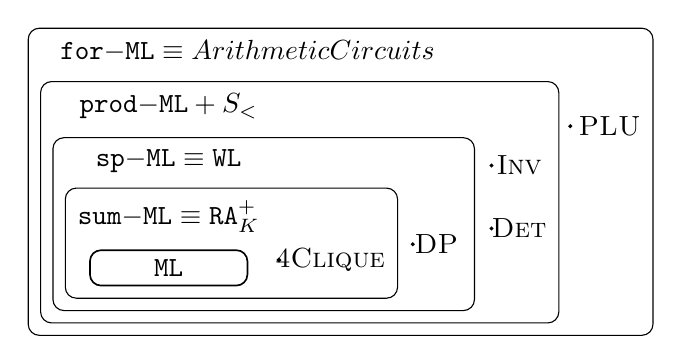
\begin{tikzpicture}[->,>=stealth, semithick, auto, initial text= {}, initial distance= {3mm}, accepting distance= {4mm}, node distance=0.5cm, semithick]
	
	\node [rectangle, draw=black, fill=white, minimum height=4mm, minimum width=2cm, rounded corners] (ML) at (0, 0) {$\texttt{ML}$};
	
	\node [inner sep=0mm] (SML) at ($(ML) + (0,0.65)$) {$\texttt{sum}\text{-}\texttt{ML}\equiv \texttt{RA}^+_K$};
	
	\node [circle, radius=4mm,draw=black, fill=black, inner sep=0mm] (pCLIQUE) at ($(ML) + (1.4,0.1)$) {};
	\node [right of=pCLIQUE,inner sep=0mm, node distance=0.65cm] (CLIQUE) {$\textsc{4Clique}$};
	
	\begin{pgfonlayer}{background}
	\node (SMLc)[draw=black, inner sep=1.5mm, rounded corners,fit=(SML)(ML)(CLIQUE)] {};
	\end{pgfonlayer}
	
	
	\node [inner sep=0mm] (sp-ML) at ($(SML) + (0,0.7)$) {$\texttt{sp}\text{-}\texttt{ML} \equiv \texttt{WL}$};
	
	\node [circle, radius=4mm,draw=black, fill=black, inner sep=0mm] (pDP) at ($(pCLIQUE) + (1.7,0.2)$) {};
	\node [right of=pDP,inner sep=0.5mm, node distance=0.3cm] (DP) {$\textsc{DP}$};
	
	
	\begin{pgfonlayer}{background}
	\node (sp-MLc) [draw=black, inner sep=1.5mm, rounded corners,fit=(SMLc)(ML)(sp-ML)(DP)] {};
	\end{pgfonlayer}
	
	
	\node [inner sep=0mm] (PML)  at ($(sp-ML) + (0,0.7)$) {$\texttt{prod}\text{-}\texttt{ML} + S_{<}$};
	
	\node [circle, radius=4mm,draw=black, fill=black, inner sep=0mm] (pINV) at ($(pDP) + (1,1)$) {};
	\node [right of=pINV,inner sep=0mm, node distance=0.35cm] (INV) {$\textsc{Inv}$};
	
	\node [circle, radius=4mm,draw=black, fill=black, inner sep=0mm] (pDET) at ($(pDP) + (1,0.2)$) {};
	\node [right of=pDET,inner sep=0mm, node distance=0.35cm] (DET) {$\textsc{Det}$};
	
	
	\begin{pgfonlayer}{background}
	\node (PMLc) [draw=black, inner sep=1.5mm, rounded corners,fit=(SMLc)(ML)(sp-MLc)(PML)(INV)(DET)] {};
	\end{pgfonlayer}
	
	
	\node [inner sep=0mm] (forML) at ($(PML) + (1,0.7)$) {$\texttt{for}\text{-}\texttt{ML} \equiv \text{Arithmetic Circuits}$};
	
	\node [circle, radius=4mm,draw=black, fill=black, inner sep=0mm] (pPALU) at ($(pINV) + (1, 0.5)$) {};
	\node [right of=pPALU,inner sep=0mm, node distance=0.5cm] (PALU) {$\textsc{PLU}$};
	
	\begin{pgfonlayer}{background}
	\node [draw=black, inner sep=1.5mm, rounded corners,fit=(SMLc)(ML)(sp-MLc)(PMLc)(forML)(PALU)] {};
	\end{pgfonlayer}
	
	\end{tikzpicture}
	
	\caption{Fragments of \langfor over square matrices and their equivalences. The functions \textsc{4Clique}, \textsc{DP} (diagonal product), \textsc{Inv}, \textsc{Det}, and \textsc{PLU} decomposition are placed in their fragments.} \label{thefigure}
\end{figure}

\section{Conclusions}\label{sec:conclude}
We proposed \langfor, an extension of \lang with limited recursion,
and showed that it is able to capture most of linear algebra due to its
connection to arithmetic circuits. We further revealed interesting connections
to logics on annotated relations. Our focus was on language design and
expressivity. An interesting direction for future work relates to efficient
evaluation of (fragments) of \langfor. A possible starting point is \cite{Christ_2013}
in which a general methodology for communication-optimal algorithms
for for-loop linear algebra programs is proposed.

\medskip
\noindent \textbf{Acknowledgements.} Mu\~noz, Riveros and Vrgo\v{c} were funded by ANID - Millennium Science Initiative Program - Code ICN17\_002.


\bibliographystyle{ACM-Reference-Format}
\balance
\bibliography{biblio}

\end{document}
\endinput
